\documentclass{article}
\usepackage{graphicx} % Required for inserting images

\usepackage[utf8]{inputenc}

\usepackage{amsmath,amsthm, amssymb}
\usepackage[margin=3cm]{geometry}
\usepackage{mathtools}
\usepackage{dsfont}
\usepackage{xcolor}
\usepackage{algorithm,algpseudocode}
\usepackage{todonotes}
\usepackage{nicefrac}
\usepackage{mathrsfs}
\usepackage{tikz}
\usepackage{authblk}

\usepackage{hyperref}


\tikzstyle{arrow} = [thick,->,>=stealth]

\usepackage{thm-restate}

\usepackage{etoc}

\usepackage{setspace}


%%%%%%%%    THEOREM DEFINITIONS AND RESTATABLE
% \newcounter{claim}
% \setcounter{claim}{0}
\newtheorem{theorem}{Theorem}
\newtheorem{lemma}[theorem]{Lemma}
\newtheorem{corollary}[theorem]{Corollary}
% \newtheorem{claim}[theorem]{Claim}
\newtheorem{definition}[theorem]{Definition}
\newtheorem{prop}[theorem]{Proposition}
% \newtheorem{assumption}{Assumption}

\usepackage{todonotes}

\newcommand{\matt}[1]{\todo[color=red!50, prepend, caption={Matt}, tickmarkheight=0.25cm]{#1}}

\newcommand{\raghav}[1]{\todo[color=blue!50, prepend, caption={Raghav}, tickmarkheight=0.25cm]{#1}}
\newcommand{\note}[1]{\emph{Note: #1}}
\newcommand{\rb}[1]{{\textcolor{blue}{RB: #1}}}

\newcommand{\conjecture}[1]{ \noindent\emph{\textbf{Conjecture:}} \emph{ #1 }}
\DeclareMathOperator{\Tr}{Tr}

\usepackage{amsthm}

%%%%%%%%    NOTATION DEFINITIONS FOR EASIER WRITING
\newcommand{\ket}[1]{|#1\rangle}
\newcommand{\bra}[1]{\langle #1|}
\newcommand{\braket}[2]{\langle #1|#2\rangle}
\newcommand{\ketbra}[2]{| #1\rangle\! \langle #2|}
\newcommand{\parens}[1]{\left( #1 \right)}
\newcommand{\brackets}[1]{\left[ #1 \right]}
\newcommand{\abs}[1]{\left| #1 \right|}
\newcommand{\norm}[1]{\left| \left| #1 \right| \right|}
\newcommand{\diamondnorm}[1]{\left| \left| #1 \right| \right|_\diamond}
\newcommand{\anglebrackets}[1]{\left< #1 \right>}
\newcommand{\overlap}[2]{\anglebrackets{#1 , #2 }}
\newcommand{\set}[1]{\left\{ #1 \right\}}
\newcommand{\divides}{\bigm|}
\newcommand{\ceil}[1]{\left\lceil #1 \right\rceil}
\newcommand{\openone}{\mathds{1}}
\newcommand{\expect}[1]{\mathbb{E}\brackets{#1}}
\newcommand{\variance}[1]{\textit{Var} \brackets{ #1 }}
\newcommand{\prob}[1]{\text{Pr}\left[ #1 \right]}
\newcommand{\bigo}[1]{O\left( #1 \right)}
\newcommand{\bigotilde}[1]{\widetilde{O} \left( #1 \right)}
\newcommand{\ts}{\textsuperscript}

\newcommand{\trace}[1]{\Tr \brackets{ #1 }}
\newcommand{\partrace}[2]{\Tr_{#1} \brackets{ #2 }}
\newcommand{\complex}{\mathbb{C}}

%%%%% COMMONLY USED OBJECTS
\newcommand{\hilb}{\mathcal{H}}
\newcommand{\partfun}{\mathcal{Z}}
\newcommand{\identity}{\mathds{1}}
\newcommand{\gue}{\rm GUE}
\DeclareMathOperator{\sinc}{sinc}
\DeclareMathOperator{\hermMathOp}{Herm}
\DeclareMathOperator{\im}{Im}
\DeclareMathOperator{\supp}{supp}
\newcommand{\herm}[1]{\hermMathOp\parens{#1}}



\title{Interpreting Multipartite Entanglement through Topological Summaries}
\author[1]{Raghav Banka}
\author[2]{Matthew Hagan}
\author[1,3,4]{Nathan Wiebe}

\affil[1]{
University of Toronto, Department of Computer Science, Toronto ON, Canada
}
\affil[2]{
University of Toronto, Department of Physics, Toronto ON, Canada
}
\affil[3]{
Pacific Northwest National Laboratory, Richland WA, USA
}
\affil[4]{
Canadian Institute for Advanced Research, Toronto ON, Canada
}



% \date{October 2023}


\begin{document}

\maketitle

\section{Introduction}
Entanglement is a hallmark feature of quantum mechanics that allows for correlations between separated systems that go beyond those allowable through classical mechanics. Although the presence of entanglement itself does not represent any kind of advantage over classical computation or communication, when entanglement is present with operations restrictions, such as only allowing arbitrary \emph{local} operations and classical communication (LOCC) between subsystems, then entanglement can become a resource. In the simulation of quantum matter, such as the electronic structure problem in chemistry or finding ground states of condensed matter systems, highly entangled ground states can pose a barrier to classical computers. Despite this importance, our understanding of entanglement is mostly based on bipartite entanglement, or quantum correlations between two halves of a single quantum system. As many quantum systems tend to have more than two constituent parties, recently efforts have been made to provide an analysis for multipartite entanglement \cite{horodecki2024multipartiteentanglement}, but an analytic treatment as complete as the bipartite case is lacking. 

\textcolor{red}{\textbf{Multipartite entanglement paragraph here.}}


Multipartite entanglement on the other hand is much less studied. In bipartite systems many questions about the entanglement structure of a state is (virtually) completely characterized by the von Neumann entropy. For multipartite systems there are much more nuanced questions that can be asked. For instance, state teleportation in multipartite systems becomes more complicated as there are no clear sources and recipients. You instead need to consider some kind of metric, such as an average or maybe a minimum fidelity across all possible bipartitions that may occur across the many subsystems. In bipartite scenarios we can declare that systems are maximally entangled if either of the reduced density matrices are maximally mixed. Loosely speaking, this tells us that the information stored in the state is across a global correlation, not locally stored in either subsystem. For multipartite states this becomes murkier. Consider the GHZ state $\ket{\rm GHZ} = \frac{1}{\sqrt{2}} \ket{00\ldots0} + \frac{1}{\sqrt{2}} \ket{1 1\ldots1}$. When looking at single subsystem the resulting state is maximally mixed, indicating some kind of global entanglement. However, when looking at a slightly larger subsystem, such as two qubits, the resulting reduced density matrix is $\rho_{1,2} = \frac{1}{2} \ketbra{00}{00} + \frac{1}{2} \ketbra{11}{11}$ which is \emph{not} maximally mixed. Even the $W$ state, characterized as $\ket{\rm W} = \frac{1}{\sqrt{3}}(\ket{100} + \ket{010} + \ket{001})$ has slightly larger von Neumann entropy for any 2 qubit reduced density matrix but many would consider the GHZ state to be more ``globally'' entangled. This raises the question of when can we consider a multipartite pure state to be ``maximally'' entangled? Further, is there even one single meaningful quantity that we can reduce multipartite entanglement to?


% \begin{align}
%     {\rm Tr}_C \ketbra{W}{W} &= {\rm Tr}_{C} \frac{1}{3}(\ket{001} + \ket{010} + \ket{100})(\bra{001} + \bra{010} + \bra{100}) \\
%     &= \frac{1}{3} (\ketbra{00}{00} + \ketbra{01}{01} + \ketbra{01}{10} + \ketbra{10}{01} + \ketbra{10}{10}).
% \end{align}



To address these questions we will follow the framework developed by Hamilton and Leditzky \cite{hamilton2023probing} which uses the seemingly unrelated area of research known as Topological Data Analysis (TDA). TDA was developed by mathematicians and computer scientists to provide insights into structural characteristics of datasets that should be independent of small noise when collecting measurements. These techniques give an overview of how many ``holes" are present in a dataset across varying distance scales. The canonical example is if we have samples of coordinates from a 3-dimensional surface it would be nice to know if the samples come from a sphere compared to a torus. TDA generalizes spheres vs tori to higher dimensions and provides a robust analysis of the number of holes across distance scales to get an idea of what features are persistent in the dataset as opposed to transient noise. Further, TDA provides a single numerical summary of the underlying manifold that data is sampled from to give a topologically invariant quantity to the data, known as the Euler's Characteristic. In graphs this corresponds to the number of edges minus the number of vertices and in three dimensional shapes it is the number of edges minus the number of vertices and minus the number of faces. This gives a quick necessary heuristic to tell if two shapes or graphs are topologically equivalent but is not sufficient to declare they are indeed the same. 

Recently Hamilton and Leditzky \cite{hamilton2023probing} showed that TDA serves as a mathematically consistent framework for studying multipartite entanglement. They showed that various entropy functionals, such as the Tsallis $q$-deformed entropy, can be used to build simplicial complexes (higher dimensional analogs of graphs) that can be fed into the TDA pipeline. One of their main results is that the resulting Euler Characteristic is exactly equal to a previously used multipartite entanglement measure known as the $n$-tangle. This not only gives a more mathematically sound justification for the use of the $n$-tangle, which was later championed in \cite{horodecki2024multipartiteentanglement} and specifically the 3-tangle, but because the Euler Characteristic is a blunt summary there remains plenty of useful topological information in the TDA pipeline. 

In this paper we continue these efforts at providing mathematically rigorous interpretations to multipartite entanglement through TDA with the goal of providing operational interpretations to the topological information. For example, in bipartite entanglement theory the entropy of entanglement between two subsystems tells us the minimum fidelity of a teleportation protocol that can be carried out between the two, or the number of bell pairs that would be needed to prepare a given bipartite state. In Section \ref{sec:prelims} we give all the necessary mathematical background and notation needed for applying TDA to multipartite quantum states. As for concrete interpretations we give operational meaning for both the Euler Characteristic as well as a characterizing result for the more fine-grained barcode data. In Section \ref{sec:distillable_entanglement} we show that the Euler Characteristic provides an upper and lower bound on the average distillable entanglement between any random bipartition of a quantum state, which can be seen as the average quantum information that can be teleported between randomly chosen parties. In Section \ref{sec:graph_states} we then analyze the barcodes that result from graph states, a fundamental primitive used in quantum communication theory and measurement based quantum computing \cite{nielsen2006} under the name of cluster states. We show that the graph state of a star graph, which is unitarily equivalent to the GHZ state, has a distinct barcode pattern. We further show that \emph{any} quantum state with such a barcode must have come from such a graph state. This shows that the GHZ state has a distinct topological fingerprint, and could be used for future verification protocols. 
 
\section{Preliminaries}\label{sec:prelims}

\subsection{Entropic Measures}
\label{subsec:entropic_measures}

We study multipartite quantum systems over a Hilbert space $\hilb_A = \hilb_{1} \otimes \hilb_{2} \otimes \ldots \otimes \hilb_{n}$, where for simplicity we will assume each individual quantum system is a qubit $\hilb_{i} = \mathbb{C}^{2}$. We will work with pure states over the total Hilbert space $\hilb_A$ or $\hilb$, denoted $\rho_A = \ketbra{\psi}{\psi}$. The reduced density operator defined over a subset $J \subseteq A$ is equal to the partial trace $\rho_J = \partrace{J^C}{\rho_A}$, where $J^C = A \setminus J$. 

% If necessary, we let $Pos(\hilb_J) \coloneqq \set{X: \hilb_J \to \hilb_J | x^\dagger X x \geq 0 ~\forall x \in \hilb_J}$ denote the set of positive semidefinite operators on a Hilbert space $H_J$ and $D(\hilb_J) \coloneqq \set{\rho \in Pos(\hilb_J) | \trace{\rho} = 1}$ the respective density operators. 

We will primarily be concerned with entropic properties, both linear and logarithmic, of reduced density operators. The standard entropy used for quantum states is the von Neumann entropy $S(\sigma) = - \trace{\sigma \log \sigma}$, where the $\log$ denotes the matrix logarithm. This matrix logarithm is fairly unwieldy to use both in practice and analytically, so we will make heavy use of either the Tsallis entropy or the Renyi divergence instead. Both provide real-valued functionals for characterizing the mixedness or uncertainty in quantum systems. The Tsallis entropies are defined for a non-zero real number $q \neq 1$ and are given by
\begin{equation}
\label{eq:tsallis_entropy}
    S_{q}(A)_{\rho} = \frac{1}{1 - q} (\trace{\rho_A^q} - 1).
\end{equation}

For $q=2$ the Tsallis entropy is equal to the purity of the state (defined as $1 - \trace{\rho^2}$) and in the limit as $q \to 1$ we have $\lim_{q \to 1} S_q(A)_{\rho} = S(\rho)$. We will omit the $\rho$ subscript from the expression when the quantum state is clear. Additionally, when referring to the entropy of a subset of the qubits in set $A$, we use $S_q(J)_{\rho} \equiv S_q(J)$ to denote the entropy of the qubits in the subset $J \subseteq A$.

% We now introduce entanglement, focusing first on the bipartite case and mentioning a few key results in the multipartite scenario.
We now introduce entanglement, focusing mostly on the bipartite case. Bipartite entanglement is a key feature of quantum mechanics and relies on a quantum state $\rho$ defined over a two party Hilbert space $\hilb = \hilb_A \otimes \hilb_B$. To define entangled states we first will describe what states are \emph{not} entangled, so-called separable states which are defined as all possible tensor products $\sigma\otimes \tau$, where $\sigma$ and $\tau$ are both valid density operators over $\hilb_A$ and $\hilb_B$ respectively. A state which is not a convex combination, or probabilistic mixture, of separable states is said to be entangled. The key notion is that a convex combination of separable states can be described as classical correlations between registers, which can be built via local unitaries performed separately on each space and classical communication between two operators of $\hilb_A$ and $\hilb_B$. A key quantity for bipartite entanglement is the entropy of entanglement, defined as $S(\rho_A) = S(\rho_B) = -\trace{\rho_B \log \rho_B}$, where $\rho_B = \partrace{\hilb_A}{\rho}$. The reason that this is a useful quantity to consider is that if $\rho$ is a pure state over the total Hilbert space $\hilb_A \otimes \hilb_B$, then the entropy of entanglement is zero if and only if the (pure!) state is separable.

After discussing what it means for quantum states to be entangled, a natural question arises: How can we measure the correlation within quantum states and differentiate states with varying degrees of entanglement?
We use measures that quantify the entanglement occurring within the quantum states with more highly entangled states receiving higher values, known as correlation measures. \rb{Maybe rephrase the current sentence and add some references} These correlation measures are crucial for operational tasks such as communication, teleportation, and cryptography. These measures must satisfy several key properties, which are clearly outlined in \cite{guhne2009entanglement}. An important aspect to highlight is the invariance of the entanglement measure under local unitary operations. Entanglement can only be generated through global operations, as local operations can only cause a basis change within individual quantum states without affecting the entanglement between subsystems. Therefore, LU(Local Unitary) equivalent quantum states have the same entanglement structure and correlation remains the same across all partitions. We will make use this property in section \ref{sec:graph_states}. These correlation measures will be useful in constructing topological structures. However, we must be careful when selecting these measures, as they need to satisfy specific properties in order to form a valid topological structure. We will discuss this further later in this section.

\rb{myabe add some references}For bipartite quantum systems, the correlation measures are well-studied, and there are many entanglement measures used in the literature, such as entanglement of formation, negativity, and relative entropy. In the bipartite scenario, we are measuring the correlation between only two subsystems. Consequently, singular value decomposition or the Schmidt rank of the quantum system effectively captures the entanglement between subsystems. However, in multipartite quantum systems, measuring correlations is difficult because the increasing number of subsystems give rise to more complex and inefficient mathematical systems defining them. In fact, the idea of maximum entanglement in such systems becomes obscure. Typically, we extend bipartite measures to make them applicable in multipartite scenarios. We will do something similar for our multipartite entanglement measure as well.

A widely used bipartite measure is the mutual information or total correlation measure which was introduced in \cite{cerf1998information}. It is defined for a composite quantum state $\rho_{AB}$ as 

\begin{equation}
\label{eq:total_correlation_bipartite}
C(A, B) = S(A) + S(B) - S(AB)
\end{equation}

This quantity is interpreted in \cite{wintercorrelations} as the minimum amount of local noise required to transform the composite entanglement system $\rho_{AB}$ into a product state $\rho_A \otimes \rho_B$ by decorrelating them. This entanglement measure can be extended to the multipartite case using the notion of relative entropy. The quantum relative entropy for density operators $\rho$ and $\sigma$ is mathematically defined as:

\begin{equation}
\label{eq:relative_entropy}
D(\rho || \sigma) = \trace{\rho \log \rho} - \trace{\rho \log \sigma} = -S(\rho) - \trace{\rho \log \sigma} 
\end{equation}
if $\supp(\rho) \subseteq \supp(\sigma)$. Otherwise the relative entropy is defined to be $+ \infty$.

Quantum relative entropy is interpreted as the ``distance" measure between two input quantum states. The mutual information measure can be expressed in terms of the relative entropy of quantum states. Specifically, the mutual information of the composite quantum state $\rho_{AB}$ is equal to the ``distance" or distinguishability between $\rho_{AB}$ and its uncorrelated counterpart $\rho_A \otimes \rho_B$ (see \cite{vderal1998relativeentropy}, \cite{vedral2002relativeentropy}), 
\begin{equation}
\label{eq:equality_of_RE_total_correlation}
    C(A, B) = D(\rho_{AB} || \rho_A \otimes \rho_B)
\end{equation}

We can define a correlation measure for multipartite quantum states by extending the quantum relative entropy to systems involving multiple parties. Let quantum state $\rho_A$ be defined over Hilbert space $\hilb_A = \hilb_{1} \otimes \hilb_{2} \otimes \ldots \otimes \hilb_{n}$. The total correlation measure of $\rho_A$ is calculated as 
 \begin{equation}
 \label{eq:multipartite_total_correlation}
     C(A_1, A_2 \dots A_n) = D(\rho_{A} || \rho_{A_1} \otimes \rho_{A_2} \dots \otimes  \rho_{A_n}) = S(A_1) + S(A_2) \dots S(A_n) - S(A)
 \end{equation}

It is important to note that relative entropy is not a true distance metric, as it is neither symmetric nor does it satisfy the triangle inequality. These properties of relative entropy are discussed in more detail in \cite{vedral2002relativeentropy}. An important feature of the total correlation measure is that it satisfies the downward property for any quantum state with a set of qubits $ A = \{A_1, A_2, \dots, A_n\} $. Specifically, for any subset $ J \subseteq K \subseteq A $, we have:
\begin{equation}
    \label{eq:downward_closure_total_correlation}
    C(J) \leq C(K)
\end{equation}
This property is a consequence of the data processing inequality of relative entropy. The data processing inequality tells us that for any quantum channel $ \Phi : \mathcal{H}_X \to \mathcal{H}_Y $ and quantum states $ \rho $ and $ \sigma $, we have:
\begin{equation}
\label{eq:data_processing_ineqaulity}
D(\Phi(\rho) || \Phi(\sigma)) \leq D(\rho || \sigma)
\end{equation}
where $ \Phi $ is a completely positive, trace-preserving linear map (see \cite{watrous2018theory}, \cite{dataprocessingnielsen} for more detailed definations). Since the partial trace can be considered a quantum channel, we can conclude that:
\begin{equation}
\label{eq:data_processing_ineqaulity_partial_trace}
D(\Tr(\rho) || \Tr(\sigma)) \leq D(\rho || \sigma)
\end{equation}

 More intuitively, $D(\rho || \sigma)$ tells how well we can distinguish between the state $\rho$ and $\sigma$. On performing partial trace over a quantum state, we are losing information about the states. Since we have less information about both states the harder it becomes to distinguish the states than before. The downward closure property \ref{eq:data_processing_ineqaulity_partial_trace} holds for the relative entropy of any two quantum states. The total correlation measure is a special case of relative entropy, where the second state is the decorrelated counterpart of the first state. Therefore, the downward closure property also holds for total correlation as well. We can prove this property of total correlation without the complications of quantum channels by simply using the subadditivity property of entropy. The proof has been provided in \cite{hamilton2023probing}.


We use the $q-$deformed correlation measure in our Topological Data Analysis depending on different values of $q$ in Tsallis entropy, as described in equation \ref{eq:tsallis_entropy}. In Section \ref{sec:distillable_entanglement}, we use on $1 - $ Tsallis entropy, and the correlation measure is defined in equation \ref{eq:multipartite_total_correlation}. The reason for choosing $q \to 1$ is to relate the topological features of the quantum state to the distillation rate of entanglement. The distillation rate corresponds more closely with the von Neumann entropy, or $1 -$Tsallis entropy, compared to other values of $q$. In Section \ref{sec:graph_states}, we go with $ q = 2 $ for Tsallis entropy, which gives us the linear entropy of entanglement. So the $2-$deformed correlation measure looks like this (similar to equation \ref{eq:multipartite_total_correlation}, but with the linear entropy):

\begin{equation}
 \label{eq:multipartite_2-deformed_total_correlation}
C_2(A_1, A_2, \dots, A_n) = S_2(A_1) + S_2(A_2) + \dots + S_2(A_n) - S_2(A)
\end{equation}

We choose $ q = 2 $ because it makes it easier to calculate the entropy of graph states, especially when using their stabilizer formalism.



\subsection{Topology Data Analysis and Notation}
\label{subsec:topology}

Topological Data Analysis (TDA) is a set of techniques for investigating properties of datasets related to their topology, or the underlying structure that the data points are drawn from. The purpose behind using topology is that the topology of a space is robust to continuous changes of the space, which when applied to data analysis means that the results drawn from TDA should be robust to significant sources of noise. TDA is of interest to the Quantum Computing community for two reasons. The predominant reason is the existence of fast quantum algorithms where no comparable classical algorithms are known. The regime for provable quantum advantages in TDA is an active area of research. The relatively recent application of TDA to quantum computing and information sciences is in revealing a link between computed topological quantities, namely the integrated Betti number, and entropic quantities of underlying quantum states on which TDA is performed. This connection between multipartite entanglement and topological data analysis is the area we explore here. 

% \rb{Need to mention the impact on topology on entanglmeny later after defining notion for topology}
To understand the impact of TDA on multipartite entanglement we first need to set our notation for the data we will be analyzing and the topological structures we will be using. Similar to techniques used in \cite{hamilton2023probing}, we consider individual qubits of multipartite quantum system as our vertices of the topological space. Let $ X^{(0)} = \{x_1, x_2, \dots, x_m\} $ be the set of distinct vertices, each representing a qubit in the input multipartite quantum state. We will primarily draw on techniques from simplicial homology, which establishes its geometric realization on simplicial complexes. A simplex is a geometric object represented uniquely by a subset of vertices from $ X^{(0)} $. More formally, an $ n-$simplex is defined as the set of $ n+1 $ distinct vertices from $ X^{(0)} $ that lie within an $ n $-dimensional space. Simplicial complexes consist of the vertex set $ X^{(0)} $ and various sets of $ n $-simplices, including  $ 1 $-simplices, up to $ (m-1) $-simplices. Additionally, simplicial complexes impose specific conditions: namely, that any subset of vertices and any non-empty intersection of simplices must also form valid simplices. Building on the concept of simplices, we define an $ n $-chain as a linear combination of $ n $-simplices. This can expressed as

$$
X^{(n-1)} = \left\{ \sum g_i \sigma_i \mid g_i \in G \right\},
$$
where $ G $ is an abelian group and $\sigma_i$ is an $n$-simplex. In this article, we take $ G $ to be the $ \mathbb{Z}_2 $ group.

Every $k$-chain complex $X^{(k)}$ takes on vector space structure with maps between them, $\partial_k : X^{(k)} \to X^{(k - 1)}$. The maps $ \partial_k $ are referred to as boundary operators, and their action on a $ k $-simplex is defined as
\begin{equation}
\partial([x_0, x_1, \cdots, x_k]) = \sum_i (-1)^i [x_0, \cdots, \hat{x_i}, \cdots, x_k],
\end{equation}
where the $ \hat{} $ operator denotes that $ x_i $ is dropped from the sequence $ [x_0, x_1, \cdots, x_k] $, see \cite{Hatcher:478079}. The action of boundary operators $\partial_k$ can be define more generally on $k$-chains using the linear property of the boundary operator $\partial_k(\sum g_i \sigma_i ) = \sum g_i \partial_k(\sigma_i )$.
This collection of vector spaces and maps is a chain complex, written as
\begin{equation}
    X^{(n)} \xrightarrow{\partial_n} X^{(n-1)} \xrightarrow{\partial_{n-1}} \ldots X^{(1)} \xrightarrow{\partial_1} X^{(0)} \xrightarrow{\partial_0} 0,
\end{equation}
if we also enforce the homology condition: $\partial_{k + 1} \circ \partial_{k} = 0$. This can be rewritten as requiring $\im \partial_{k + 1} \subset \ker \partial_{k}$. As $\im \partial_{k + 1}$ and $\ker \partial_{k}$ are subspaces of the vector space $X^{(k)}$, we can consider the quotient space $ H_{k} \coloneqq  \frac{\ker \partial_{k}}{\im \partial_{k + 1}}$, which is called the $k$\ts{th} homology group. Its dimension as a vector space is an important number, the $k$\ts{th} Betti number $\beta_k \coloneqq \dim(H_k) = \dim(\ker \partial_k) - \dim(\im \partial_{k + 1})$. The alternating sum of these Betti numbers gives the Euler Characteristic 
\begin{equation}
    \chi = \sum_{i = 0}^{k} (-1)^i \beta_i.
\end{equation}

To better understand the TDA pipeline, readers can refer to Figure \ref{fig:enter-label}. The analysis begins with a quantum state as input. The TDA process starts by calculating the entropy of the marginals of the input quantum state to construct simplices. For every subset of qubits in the input quantum state, we define correlation functions that map these sets of vertices to real numbers. In Section \ref{sec:distillable_entanglement}, we employ the total correlation measure as our functional, while for Section \ref{sec:graph_states}, we use the linear entropic correlation measure. Both of these functionals act as metric to quantify the degree of correlation in quantum states. We construct a simplex for a set of vertices $A$ if the correlation function $C(A)$ satisfies $C(A) \leq \epsilon$, where $\epsilon$ is a filtration parameter. As we gradually increase $\epsilon$ from 0 to $\epsilon_{\text{max}}$, the set of vertices $A$ that satisfy the condition $C(A) \leq \epsilon$ forms a simplex at each step. These correlation measures possess the downward closure property, meaning that the correlation function is monotonic under partial traces, also discussed in \ref{subsec:entropic_measures}. Therefore, if a set of vertices $A$ satisfies $C(A) \leq \epsilon$, then any subset of $J \subseteq A$ will also satisfy the condition $C(J) \leq \epsilon$, ensuring that any subset of $A$ also forms a simplex. This property is crucial for the structure of simplices, as it guarantees that every non-empty proper subset of a simplex is also a valid simplex. We halt our analysis when the entire topological space forms a single simplex. The filtration parameter where we stop our computation is denoted $\epsilon_{max}$. Using these simplices, we can extract topological features such as Betti numbers and the Euler characteristic. While we have an intuitive understanding of these topological characteristics, developing a concrete method for interpreting them remains an open question. 

The Betti numbers and Euler characteristic are the main homological quantities we will use to get a quantitative estimate of the ``connectedness" of a simplicial complex $X$. The $0$-dimensional holes in the topological structure represent the number of connected components. If $X$ has a large $\beta_0$ this tells us there are a lot of disconnected pieces of the complex. A large $\beta_1$ tells us there are a lot of one-dimensional holes(corresponding to cycles) in the complex, similar to gluing a bunch of donuts together to tile a big square.  In contrast to traditional techniques in topological data analysis (TDA), persistent homology tracks the lifespan of holes—specifically, their birth and death times. The intuition behind this approach is that the persistence of a hole reflects the ``significance" of noise in the dataset. In other words, holes that persist longer correspond to more ``important" defects in the dataset and vice versa. Persistent homology provides richer insights into the dataset, particularly by revealing the lifespan of holes. Higher-dimensional Betti numbers are computationally expensive and challenging to analyze. In this paper, we aim to provide an application of lower-dimensional Betti numbers in understanding the global quantum state.


Another application application of topology is to capture the fundamental skeletal structure of shapes. To quantify these structures, we use topological invariants like the Euler characteristic, which remains constant under bending and stretching of the shape, preserving its essential form. We will be performing our analyses using persistent homology, explained rigorously in \cite{hamilton2023probing}. We extend the notion of Euler characteristic to the reduced integrated Euler characteristic (IEC), denoted by $\tilde{\mathfrak{X}}$, which is again formally defined in \cite{hamilton2023probing}. This quantity is sum the Euler characteristic up to $\epsilon_{max}$. In the same paper, the authors Hamilton and Leditzky demonstrated that the IEC of multipartite quantum states is equivalent to the interaction information of the quantum state. We build upon this work to present an operational interpretation of the IEC of the quantum system.

% Now we explain the simplicial complexes we will construct and the topological data analysis pipeline. 

% Traditionally, in TDA using victoria rips complex, we  points in $X^{0}$ we construct a line, or edge, between $(x_i, x_j) \in X^{(1)}$ if $d(x_i, x_j) \leq \epsilon$, where $\epsilon$ is a length scale that filters out far apart nodes. 

% In our analysis, we use functionals that map sets of vertices to real numbers. For Section \ref{sec:distillable_entanglement}, we employ the total correlation measure as our functional, while for Section \ref{sec:graph_states}, we use the linear entropy. Both of these functionals measure the degree of correlation in quantum states. We construct a simplex for a set of vertices $A$ if the correlation function $C(A)$ satisfies $C(A) \leq \epsilon$, where $\epsilon$ is a filtration parameter. As we gradually increase $\epsilon$ from 0 to $\epsilon_{\text{max}}$, the set of vertices $A$ that satisfy the condition $C(A) \leq \epsilon$ forms a simplex at each step. These correlation measures possess the downward closure property, meaning that the correlation function is monotonic under partial traces, also discussed in \ref{subsec:entropic_measures}. In other words, if a set of vertices $A$ satisfies $C(A) \leq \epsilon$, then any subset of $J \subseteq A$ will also satisfy the condition $C(J) \leq \epsilon$, ensuring that the set form a simplex. This property is crucial for the structure of simplices, as it guarantees that every non-empty proper subset of a simplex is also a valid simplex. 

% We construct topological simplices based on the entanglement of a subset of qubits. The $0$-dimensional holes in the topological structure represent the number of connected components. At a filtration parameter $\epsilon$, if two vertices are not connected, they contribute to the $0$-th Betti number. From our construction of simplices, we know that if two points are not connected, the correlation measure between them exceeds $\epsilon$. Thus, a high persistence of less $0$-dimensional holes indicates a strong correlation between pairs of vertices in the topological structure. In other words, the more disconnected the structure remains, the greater the entanglement between pairs of points.

% The starting point of the TDA pipeline is the data, represented as a collection of points $\mathcal{D} = \set{x_i : 1 \leq i \leq n, x_i \in \mathcal{X}}$, where the only structure we need on the space $\mathcal{X}$ is the ability to compute a distance between points $d(x, y)$. 

% Once we have this dataset we then can construct the simplicial complex $X(\epsilon)$ we will compute the homology of. There are two ways to construct this complex, the Vietoris-Rips method and the Cech method. For starters we will stick to the computationally simpler Vietoris-Rips method. The Vietoris-Rips complex $X$ has one node per point $x_i$ in $\mathcal{D}$. From these points we construct a line, or edge, between $(x_i, x_j) \in X^{(1)}$ if $d(x_i, x_j) \leq \epsilon$, where $\epsilon$ is a length scale that filters out far apart nodes. Later we will show how changing $\epsilon$ gives TDA it's power, but for the purposes of illustrating the pipeline we will consider a fixed $\epsilon$ and typically drop the implicit parametrization $X(\epsilon) = X$. Once we have the edges of $X^{(1)}$ we fill in an element $(x_i, x_j, x_k)$ in the next dimension $X^{(2)}$ if and only if these nodes form a clique in $X^{(1)}$, meaning all edges $(x_i, x_j), (x_i, x_k),$ and $(x_j, x_k)$ are present in $X^{(1)}$. We then proceed to higher dimensions, filling in a simplex if there is a clique present in $X^{(1)}$. Clique finding is a notoriously difficult problem without an upper bound on the size of cliques to check, so we put a cap on the dimension $n$, or cliques of size $n + 1$ nodes.

% \begin{figure}
%     \centering
%     \begin{tikzpicture}[main/.style = {draw, rectangle}] 
%             \node[main] (1) at (0, 3) {Weighted graph $G$};
%             \node[main] (2) at (0, 0) {Simplicial Complex $X$};
%             \node[main] (3) at (5.75, 3) {Betti Numbers $\beta_i$};
%             \node[main] (4) at (5.75, 0) {Euler Characteristic $\chi$};
%             \draw [arrow] (1) -- node[left]{Filtration $\epsilon$}(2);
%             \draw [arrow] (2) -- node[left]{$\dim \ker \Delta_i(\epsilon)$} (3);
%             \draw [arrow] (3) -- node[right]{$\sum_i (-1)^i \beta_i(\epsilon)$} (4);
%         \end{tikzpicture}
%     \caption{Basic TDA pipeline}
%     \label{fig:enter-label}
% \end{figure}
\begin{figure}
    \centering
    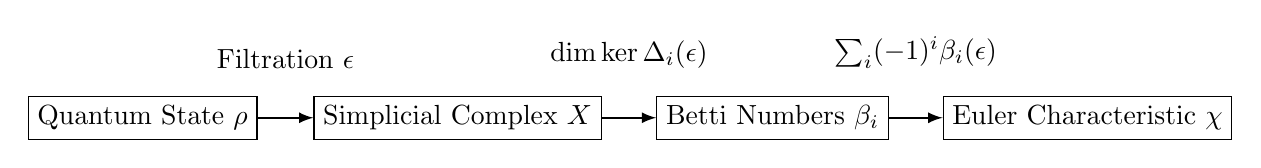
\begin{tikzpicture}[main/.style = {draw, rectangle}] 
        \node[main] (1) at (0, 0) {Quantum State $ \rho $};
        \node[main] (2) at (4, 0) {Simplicial Complex $ X $};
        \node[main] (3) at (8, 0) {Betti Numbers $ \beta_i $};
        \node[main] (4) at (12, 0) {Euler Characteristic $ \chi $};
        \draw[->, thick, >=latex] (1) -- node[above, yshift=0.5cm]{Filtration $ \epsilon $} (2);
        \draw[->, thick, >=latex] (2) -- node[above, yshift=0.5cm]{$ \dim \ker \Delta_i(\epsilon) $} (3);
        \draw[->, thick, >=latex] (3) -- node[above, yshift=0.5cm]{$ \sum_i (-1)^i \beta_i(\epsilon) $} (4);
    \end{tikzpicture}
    \caption{Basic TDA pipeline}
    \label{fig:enter-label}
\end{figure}



% \subsection{Simplicial complexes} \label{sec:simplicial_defs}

% We will be working with simplicial complexes and homological constructions, so should give some simple definitions. Let $X^{(0)} = \set{x_1, x_2, \ldots, x_n}$ denote the set of vertices.  
% \begin{definition}[Simplicial Complex] \label{def:simplicial_complex}
%     A (abstract) simplicial complex defined over a set of points $X^{(0)}$ is a collection $X$ of subsets of $X^{(0)}$ such that if $\tau \in X$ and $\sigma \subseteq \tau$ then $\sigma \in X$. 
% \end{definition}

% \begin{definition}[n-simplex $\Delta ^ n$] \label{def:n-simplex}
%     A geometric figure determined by a collection of $n + 1$ points in Euclidean space $\mathbb{R}^n$. It is defined as a complete graph on $n+1$ vertices or a n-dimensional clique.
% \end{definition}

% Generally in Homology a n-simplex is formed when $n + 1$ points in Euclidean space $\mathbb{R}^n$ forms a clique, ie when every n-1 simplex contained in the n simplex is formed. However, In this paper \cite{hamilton2023probing} A simplex is formed only when the filtration parameter $\epsilon$ is greater than the functional $F(\rho)$ ie $F(\rho) \leq \epsilon$. We can think of simplex formation as subsets of  $X^{(0)}$ being added to a collections. There are n collections: One collection to contain subsets of size ranging from $1$ to $n$. Sometimes we write n-simplex as $[x_0, .., x_n]$ where $x_i$ are the vertices belonging to the n-simplex

% \begin{definition}[Face of simplex] \label{def:n-simplex}
%     Given a n-simplex $[x_0, .., x_n]$, we have the simplex containing $n+1$ points. If we delete an arbitrary point from n-simplex then we are left with n points which form a $n$ points which form a $n-1$-simplex following the definition 2 of a simplicial complex. This $n-1$ simplex formed is called the face of the n-simplex
% \end{definition}

% In \cite{hamilton2023probing}, we are using a functional $F(\rho)$ on subset of vertices and filtration parameter $\epsilon$ such that subset of vertices form a simplex when $F(\rho) \leq \epsilon$. Since every face of a n-simplex is also a simplex we want every face of the n-simplex to form a simplex before the n-simplex is formed. This requires monotonicity from the functional F such that $F(I) \leq F(J) $ for $I \subseteq J$  

% \begin{definition}[n-chain] \label{def:n-chain}
%     Let $A_1^n, A_2^n, A_3^n, ... A_k^n$ be arbitrary oriented n-simplices of a complex K and an abelian group G, we define an n-chain x with coefficients in G as a formal sum:
%     $$x = g_1 \cdot A_1^n + g_2 \cdot A_2^ n + g_3 \cdot A_3^ n + ... g_k \cdot A_k^ n $$
%     where $g_i \in G$.
%     In most cases $G = Z$. However for our purposes and for the sake of simplicity, we assume $G = \{0, 1\}$ or $Z_2$. Let $L_n$ be the group of n-chains
% \end{definition}

% \begin{definition}[Boundary of n-simplex] \label{def:Boundary of n-simplex}
%     Let $A^n$ be an oriented n-simplex in a complex K. The boundary of $A^n$ is defined as the $n - 1$ chain of K over abelian group G given by 
%     $$\delta(A^n) = A_0^{n-1} + A_1^{n-1} + A_2^{n-1} ... + A_n^{n-1}$$
%     where $A_i^{n-1}$ is a n-1 face of n-simplex $A^n$. 
%     \\ The boundary of $A^n$ is given by n+1 number of $n - 1$ simplex.
% \end{definition}
% \begin{definition}[Boundary of n-chain] \label{def:Boundary of n-chain}
%     For any n-chain, $l = \Sigma_{i=1}^{i=k} g_i \cdot A_i^{n}$ we define the boundary of chain to to be 
%     \begin{equation}
%         \delta(l) =   \sum_{i=1}^{i=k} g_i \cdot \delta(A_i^{n})
%     \end{equation}
%     where $A_i^{n}$ are the n-simplexes of K. Therefore, the boundary operator $\delta$ is a homomorphism $\delta$ : $L_n \xrightarrow{} L_{n-1} $
% \end{definition}
% \begin{definition}[Cycle] \label{def:Cycle}
%     When an n-chain has boundary 0, the n-chain is considered a cycle. It is represented as the $Ker(\delta)$
% \end{definition}
% \begin{definition}[Homology Group $H_n$] \label{def:Homology Group}
%     We define the homology Group $H_n = Ker(\delta) / Im(\delta)$
% \end{definition}
% \begin{definition}[kth Betti Number] \label{def:kth Betti Number}
%     We define the kth Betti Number as the rank of the kth homology Group, ie $B_k = rank(H_k)$
% \end{definition}
% \begin{definition}[Euler Characteristic] \label{def:Euler Characteristic}
%     This has two definitions first based on the betti number and another based on the number of simplicial complex. 
%     \begin{equation}
%         \chi = \sum_i (-1)^i \cdot B_i
%     \end{equation}
%     Let $n_k$ be the number of k-simplices.
%     \begin{equation}
%         \chi = \sum_i (-1)^i \cdot n_i
%     \end{equation} 
    
% \end{definition}

% \subsection{Preliminaries}
% Assume Graph $G = (V, E)$ to have least 4 vertices and no isolated vertex. Denote $\ket{G}$ as graph state corresponding to graph $G$. For any vertex set $A \subseteq V$, the reduced density matrix $ \rho^A_G $ is defined as:
% $
% \rho^A_G = \Tr_{V \setminus A} \left( \ket{G} \bra{G} \right)
% $. 
% The linear entropy (Second Tsallis entropy) of the reduced density operator $\rho^A_G$, represented by $S_2(\rho^A_G) \equiv S_2(A)$, is defined as
% \begin{align} \label{eq:linear_entropy}
% S_2(A) &= 1 - \Tr\left((\rho^A_G)^2\right) \\
%        &= 1 - \sum_{i} \lambda(i)^2  
% \end{align}
% where $ \lambda(i) $ denotes the $ i $-th eigenvalue of the reduced density matrix $ \rho^A_G $, with the eigenvalues of $ \rho^A_G $ ordered as $ \lambda_1 \geq \lambda_2 \geq \cdots \geq \lambda_d $.

% The 2-deformed correlation function of the reduced density matrix $\rho^A_G $, denoted by $ C_2(\rho^A_G) \equiv C_2(A)$, is computed as:
% \begin{equation}
% \label{eq:correlation_function}
% C_2(A)  = \sum_{v \in A} S_2(v) - S_2(A).    
% \end{equation}


\section{Entanglement Distillation} \label{sec:distillable_entanglement}
Quantum gate (or state) teleportation is a foundational protocol in Quantum Computing and information sciences. In Quantum Computing, T-gates are teleported from so called ``magic state" factories to be used to implement T-gates within the operation of an error-correcting code. This is crucial to avoid the Easton-Knill Theorem, which states that the logical operations available to implement transversally (meaning the operation acts on the encoded quantum state) are \emph{not} fully universal and that the two routes to avoid this are to either switch from one quantum code to another, such that all gates can be done, or to create resource states outside of the quantum code and use gate teleportation to apply the gate. Utilizing gate teleportation is a much simpler route that most fault-tolerant research analyzes. Behind this crucial operation of teleportation lies a  primitive known as a Bell pair, which is a pair of entangled qubits in one of the following four states
\begin{equation}
    \frac{\ket{0}\ket{0} \pm \ket{1}\ket{1}}{\sqrt{2}}, \frac{\ket{0}\ket{1} \pm \ket{1}\ket{0}}{\sqrt{2}}. 
\end{equation}
In this section we explore how the number of such pairs that can be extracted, called the Distillable Entanglement, from bipartitions of a multipartite state is related to the Integrated Euler Characteristic (IEC) of an entanglement complex derived from the multipartite state.

Consider a global pure state $\rho = \ketbra{\psi}{\psi}$ over our Hilbert space $\mathcal{H} = (\mathbb{C}^2)^{\otimes n}$ and suppose that we split the state in half, giving a subset $A \subsetneq S$ of qubits to Alice and $B = S \setminus A$ to Bob. Denote their respective states $\rho_A = \Tr_B ( \ketbra{\psi}{\psi})$ and $\rho_B$ similarly. Now imagine the global state happens to be a product state across this bipartition, so $\rho = \rho_A \otimes \rho_B$. No matter what LOCC channels Alice or Bob apply, they will never be able to share a Bell pair between themselves. On the complete opposite end of the spectrum, if the global state is equal to a tensor product of Bell pairs $\rho = \left(\frac{\ket{0}\ket{0} + \ket{1}\ket{1}}{\sqrt{2}} \right)^{\otimes n} \left(\frac{\bra{0}\bra{0} + \bra{1}\bra{1}}{\sqrt{2}} \right)^{\otimes n}$, then we can split up each of the pairs, giving one half to Alice and the other to Bob, and without doing any LOCC they will share $n$ Bell pairs. This number is called the distillable entanglement $E_D$ and it is defined as the upper limit to how many Bell pairs Alice and Bob can create using their part of the state $\rho$, along with LOCC channels. This is defined formally below. 

% \textbf{General Idea}: Does the Integrated Euler characteristic(IEC) tell us anything about the Entanglement distillation \\
% Consider an arbitrary pure state $\ket{\psi}$ lying in Hilbert space $\mathcal{H}$. The corresponding density operator is $\rho = \ket{\psi}\bra{\psi}$.
% We partition the quantum system $\rho$ into two subsystems, A and B, such that their combined state resides in the Hilbert space  $\mathcal{H} = \mathcal{H_A} \otimes \mathcal{H_B}$. The reduced states $\rho_A = \Tr_B(\ket{\psi}\bra{\psi})$ and $\rho_B = \Tr_A(\ket{\psi}\bra{\psi})$ are then sent to Alice and Bob, respectively, each having access only to their state. They are allowed to perform any unitary transformations and measurements, on their respective subsystems and can coordinate their actions through rounds of classical communication (LOCC). Given multiple copies of their respective system, Alice and Bob convert their input to the maximum number of singlets possible.

% The composite quantum state $\rho$, partitioned into subsystems A and B, is represented as $\rho_{AB}$. Given Alice and Bob gets subsystem $\rho_A$ and $\rho_B$ respectively, the maximum number of singlets Alice and Bob can distill using LOCC is represented by $E_D(\rho_{AB})$. In a multi-party scenario, the original state can be partitioned and singlets distilled in several ways by sending observers Alice and Bob different partitions. We introduce the quantity called the average entanglement distillation rate, $\langle E_D \rangle$, which represents the average rate of entanglement distillation across all possible partitions of the multipartite input state. We show that the integrated Euler characteristic can be both upper and lower bounded by the quantity $\langle E_D \rangle$, thereby revealing a connection between Topological Data Analysis and the distillation rate.

\begin{definition} [Distillable Entanglement $E_D(\rho_{AB})$]
Let $\rho = \ketbra{\psi}{\psi}$ be a pure quantum state over a Hilbert space $\mathcal{H}$ with a bipartition $\mathcal{H} = \mathcal{H}_A \otimes \mathcal{H}_B$. Let $\Phi_{A \times B}^{(n)} \in LOCC((\mathcal{H}_A \otimes \mathcal{H}_B)^{\otimes n})$ be a family of ``distilling" channels that utilize only LOCC operations between asymptotically many copies of $\mathcal{H}_A$ and $\mathcal{H}_B$ that aim to create copies of Bell pairs $\tau = \left(\frac{\ket{0}\ket{0} + \ket{1}\ket{1}}{\sqrt{2}} \right) \left(\frac{\bra{0}\bra{0} + \bra{1}\bra{1}}{\sqrt{2}} \right)$. The \emph{distillable entanglement} is then the supremum value of all integers $m$ such that 
$$
\lim_{n \to \infty} F\left( \tau^{\otimes m}, \Phi_{A \times B}^{(n)} (\rho^{\otimes n}) \right) = 1.
$$

% is defined the maximum rate at which singlet states can be distilled from an asymptotically large copies of the arbitrary input quantum state $\rho$ using a Local Operations and Classical Communication (LOCC) protocol.
% \begin{equation} 
%     E_D(\rho) = \sup_{LOCC} \lim_{n \rightarrow \infty} \frac{m}{n}
% \end{equation}
% The LOCC protocol maps n copies of input state $\rho$ to m copies of output singlet states
% \end{definition}
% \begin{definition} [Entanglement Cost $E_C(\rho)$)]
%     Entanglement Cost is defined as the minimum rate at which asymptotic copies of singlet states can be transformed to an arbitrary output state $\rho$ using a Local Operations and Classical Communication (LOCC) protocol.  
% \begin{equation}
%     E_C(\rho) = \inf_{LOCC} \lim_{n \rightarrow \infty} \frac{m}{n}
% \end{equation}
% The LOCC protocol maps n copies of input singlet state to m copies of output state $\rho$
\end{definition}
\begin{definition} [Average Distillable Entanglement]
    Let $\rho = \ketbra{\psi}{\psi}$ be a pure multipartite quantum on Hilbert space $\mathcal{H}_A = \mathcal{H}_{\mathcal{A}_1} \otimes \mathcal{H}_{\mathcal{A}_2} \otimes \dots \otimes \mathcal{H}_{\mathcal{A}_n}$  where $\mathcal{A} := \{\mathcal{A}_1, \ldots \mathcal{A}_n\}$. The average distillable entanglement is the mean value of the distillable entanglement calculated over all possible bipartitions of $\mathcal{H_A} = \mathcal{H}_J \otimes \mathcal{H}_{J^c}$ where $J \subseteq A$ and $J^c = A \setminus J$
    \begin{equation}
     \langle E_D \rangle = \frac{\sum_{\substack{J \subseteq \mathcal{A}} }E_D(\rho_{J J^{C}})}{2^n}.
    \end{equation}
    
\end{definition}
\begin{theorem}
\label{theroem:euler_characteristic_distillation}
Let $\rho = \ketbra{\psi}{\psi}$ be a pure multipartite quantum state on Hilbert space $\mathcal{H}_A = \mathcal{H}_{\mathcal{A}_1} \otimes \mathcal{H}_{\mathcal{A}_2} \otimes \dots \otimes \mathcal{H}_{\mathcal{A}_n}$  where $\mathcal{A} := \{\mathcal{A}_1, \dots \mathcal{A}_n\}$. The reduced Integrated Euler characteristic $\tilde{\mathfrak{X}}(\infty)$ of the persistence module created using functional $C(J)_\rho = \sum_{v \in J} S(v)_\rho - S(J)_\rho$ for $J \subseteq A$ is bounded below and above by,
\begin{equation}
\langle E_D \rangle - \frac{1}{2} \epsilon_{\text{max}}  \leq \frac{\tilde{\mathfrak{X}}(\infty)}{2^n} \leq \langle E_D \rangle
\end{equation}
where $\langle E_D \rangle$ is the average distillable entanglement of $\rho$ and $\epsilon_{max}$ is that maximum filtration parameter where the barcodes of persistence module stops changes.
\end{theorem}
\begin{proof}
For pure states $\rho_{AB}$, Ref.\cite{bennet_distillation} showed that the entanglement distillation rate, when partitioning the state $\rho$ into subsystems $A$ and $B$, can be quantified by the entropy of entanglement, given by
\begin{equation}
\label{eq:Distillation_Cost_Equality}
     E_D(\rho_{AB}) = S(\rho_A) = -\Tr(\rho_A \log \rho_A)
\end{equation}
where $\rho_A = \Tr_B(\ket{\psi}\bra{\psi})$. For reduced density state $\rho_A$, the von Neumann entropy is denoted as $S(A)_\rho \equiv S(\rho_A)$.

Let $\rho$ be a pure quantum state over Hilbert space $\mathcal{H}_{\mathcal{A}} $. The Hilbert space $ \mathcal{H}_{\mathcal{A}} $ is defined as $ \mathcal{H}_{\mathcal{A}_1} \otimes \mathcal{H}_{\mathcal{A}_2} \otimes \dots \otimes \mathcal{H}_{\mathcal{A}_n} = (\mathbb{C}^2)^{\otimes n} $ where $\mathcal{A} := \{\mathcal{A}_1, .... \mathcal{A}_n\}$. According to Theorem 4.18 in  \cite{hamilton2023probing}, the reduced integrated Euler characteristic is given as a sum over subsets of the total Hilbert space as
% \setlength{\jot}{5pt}
\begin{flalign}
    \tilde{\mathfrak{X}}_q(\infty) &=  \sum_{J \subseteq  \mathcal{A}} (-1)^{|J| - 1} S_q(J)_{\rho}.
\end{flalign}
As $q \rightarrow 1$, Tsallis entropy defined as $S_q(J)_{\rho}$ approaches the von Neumann entropy, $\lim_{q \rightarrow 1} S_q(J)_{\rho} = S(J)_{\rho} = -\Tr(\rho_J \log \rho_J)$. Using von Neumann entropy formalism in previous equation, 
\begin{flalign}
   \tilde{\mathfrak{X}}(\infty) &=  \sum_{J \subseteq  \mathcal{A}} (-1)^{|J| - 1} S(J)_{\rho}  \\
    \label{eq:IEC_rearranged}
    \tilde{\mathfrak{X}}(\infty) &=  \sum_{\substack{J \subseteq \mathcal{A}}}  S(J)_{\rho} - 2 \sum_{\substack{J \subseteq \mathcal{A} \\ |J| \text{mod} 2 = 0}}  S(J)_{\rho} 
\end{flalign}
Dividing equation $\eqref{eq:IEC_rearranged}$ by $2^n$, we get
\begin{flalign}
    \frac{\tilde{\mathfrak{X}}(\infty)}{2^n} &= \frac{\sum_{\substack{J \subseteq \mathcal{A}}}  S(J)_{\rho}}{2^n} - \frac{1}{2^{n-1}}\sum_{\substack{J \subseteq \mathcal{A} \\ |J| \text{mod} 2 = 0}}  S(J)_{\rho} 
\end{flalign}
Substituting in equation \eqref{eq:Distillation_Cost_Equality} in our previous equation, we get
\begin{flalign}
    \frac{\tilde{\mathfrak{X}}(\infty)}{2^n} &= \frac{\sum_{\substack{J \subseteq \mathcal{A}} }E_D(\rho_{J J^{C}})}{2^n} - \frac{1}{2^{n-1}} \sum_{\substack{J \subseteq \mathcal{A} \\ |J| \text{mod} 2 = 0}}  S(J)_{\rho}  
\end{flalign}
where $J^{C} = \mathcal{A} \setminus J$
\begin{flalign}
    \label{eq:IEC_avgDistillation_equality}
    \frac{\tilde{\mathfrak{X}}(\infty)}{2^n} &= \langle E_D \rangle - \frac{1}{2^{n-1}}\sum_{\substack{J \subseteq \mathcal{A} \\ |J| \text{mod} 2 = 0}}  S(J)_{\rho}   \\
     \frac{\tilde{\mathfrak{X}}(\infty)}{2^n} & \leq \langle E_D \rangle
\end{flalign}
as von Neuman Entropy is non-negative, ie $S(J)_\rho \geq 0$ for any $J \subseteq \mathcal{A}$.

The total correlation function for a multipartite quantum state $ \rho $ defined on the set $\mathcal{A} := \{ A_1, .... A_n \}$ is defined as 
\begin{equation}
    C(\mathcal{A})_{\rho} = \sum_{v \in \mathcal{A}} S(v)_{\rho} - S(\mathcal{A})_{\rho} 
\end{equation}
On rewriting the equation, entropy of the system on set $\mathcal{A}$ can be written in terms of the entropy of individual subsystems and correlation function
\begin{equation}
    \label{eq:entropy_in_terms_of_correlation}
    S(\mathcal{A})_{\rho} = \sum_{v \in \mathcal{A}} S(v)_{\rho} -  C(\mathcal{A})_{\rho}
\end{equation}
Substituting in eq \eqref{eq:entropy_in_terms_of_correlation} into eq \eqref{eq:IEC_avgDistillation_equality} yields the following result
\begin{flalign}
    \frac{\tilde{\mathfrak{X}}(\infty)}{2^n} &= \langle E_D \rangle - \frac{1}{2^{n-1}}\sum_{\substack{J \subseteq \mathcal{A} \\ |J|\!\!\!\! \mod 2 = 0}} \left( \sum_{v \in J} S(v)_{\rho} -  C(J)_{\rho} \right) 
\end{flalign}
For an element $v \in A$, the number of even-length subsets that include $v$ can be determined by considering the remaining $n - 1$ elements. Odd-length subsets of the remaining $n-1$ elements are obtained by including v as an element in the set. The number of odd-length subsets of a set with $n-1$ elements is given by: $\sum_{k \mod 2 = 1} \binom{n - 1}{k} = 2^{n-2}$.
\begin{flalign}
    \frac{\tilde{\mathfrak{X}}(\infty)}{2^n} &= \langle E_D \rangle - 2^{n-2} \cdot \frac{1}{2^{n-1}}\sum_{v \in \mathcal{A}}  S(v)_{\rho} + \frac{1}{2^{n-1}} \sum_{\substack{J \subseteq \mathcal{A} \\ |J| \!\!\!\!\mod 2 = 0}}  C(J)_{\rho} \nonumber\\
    &=\langle E_D \rangle - \frac{1}{2}\sum_{v \in \mathcal{A}}  S(v)_{\rho} + \frac{1}{2^{n-1}} \sum_{\substack{J \subseteq \mathcal{A} \\ |J| \!\!\!\!\mod 2 = 0}}  C(J)_{\rho}
\end{flalign}
The correlation function is non-negative, a result that follows from the property of subadditivity. By omitting the correlation function from the previous equation, we obtain
\begin{flalign}
    \frac{\tilde{\mathfrak{X}}(\infty)}{2^n} & \geq \langle E_D \rangle - \frac{1}{2} \sum_{v \in \mathcal{A}}  S(v)_{\rho} 
\end{flalign}
Based on the definition provided in \cite{hamilton2023probing},  $\epsilon_{max}$ as the largest value of the filtration parameter at which the number of barcodes changes. For any pure quantum state $ \rho $ defined on the set $ \mathcal{A} $, $ \epsilon_{\text{max}} = \sum_{v \in \mathcal{A}} S(v)_{\rho} $. At this value of $ \epsilon_{\text{max}} $, the entire topological structure forms a simplex, resulting in the collapse of the barcode into a single 0-dimensional hole. The lower bound can be defined in terms of average entanglement distillation and $\epsilon_{\text{max}}$,
\begin{flalign}
    \frac{\tilde{\mathfrak{X}}(\infty)}{2^n} & \geq \langle E_D \rangle - \frac{1}{2} \epsilon_{\text{max}} 
\end{flalign}
\end{proof}
Theorem \ref{theroem:euler_characteristic_distillation} provides an insightful operational interpretation of the topological features of a quantum state. By bounding the IEC with the average distillation rate across possible partitions, we have a potential method for quantifying and predicting the efficiency of quantum state purification. A more mathematical interpretation of the theorem is that when calculating the distillation rate of a multipartite quantum state over statistically distributed partitions, the average distillation rate will be bounded by the Integrated Euler's Characteristic (IEC) of the quantum state. The IEC encapsulates the broader, global characteristics of the quantum state, and this result emphasizes how these global features influence local purification operations. The primary objective behind this result was to investigate more operational applications of topology within quantum information theory.

\subsection{$k-$uniform states}
We will now discuss the applications of the average distillable entanglement introduced earlier. A similar entanglement measure has been studied in previous works, such as in \cite{Scott_k-uniform} and \cite{meyer2001global}. In \cite{Scott_k-uniform}, the authors used the linear entropy measure instead of the von Neumann entropy that we have employed. Both entropic measures—those discussed here and in previous works—share the same core principle: they calculate the average entropy across all partitions of a multipartite quantum system. These measures have been used to identify a particular class of quantum states known as $k$-uniform states. This special class of quantum states has been studied under various labels, such as $k$-MM states \cite{Cerf_k-MM}, $k$-uniform states, and normal forms \cite{MoorNormal_form}. These states are useful in studying quantum error correction codes\cite{Scott_k-uniform}, characterizing entanglement \cite{meyer2001global}, and analyzing the effects of local unitary operations in quantum systems \cite{Kraus_LU_Equivalence}. In fact the construction of such quantum states have been an open problem for study in information theory \cite{Karol_k-uniform_construction}. A specific type of $k$-uniform system, known as the Absolutely Maximally Mixed State (AME), is a $\lfloor \frac{n}{2} \rfloor$-uniform state. Because of its highly entangled structure, this class of quantum state has proven to be highly important in ADS/CFT protocols, holographic codes \cite{preskill_holographic_codes}, secret sharing \cite{Helwig_AME}, and teleportation protocols \cite{Helwig:2013ckb}. We will now define $k$-uniform quantum systems and discuss how they relate to our entanglement measure of average distillable entanglement.

\begin{definition}
\label{def:k-uniform}
($k$-uniform state)
    Let $\rho = \ketbra{\psi}{\psi}$ be a pure multipartite quantum state on Hilbert space $\mathcal{H}_A = \mathcal{H}_{\mathcal{A}_1} \otimes \mathcal{H}_{\mathcal{A}_2} \otimes \dots \otimes \mathcal{H}_{\mathcal{A}_n} = (\mathbb{C}^2)^{\otimes n}$  where $\mathcal{A} := \{\mathcal{A}_1, \ldots \mathcal{A}_n\}$. We say that the quantum state $\rho$ is $k-$uniform if 
    \begin{equation}
        \rho_J = \rho_{J^c} = \Tr_{J^c}(\ketbra{\psi}{\psi}) = \frac{\identity}{2^k}
    \end{equation}
for each non empty subset $ J \subset \mathcal{A} $ with $ |J| = k $, and where $ J^c \coloneqq \mathcal{A} \setminus J $, the possible values of $ k $ range from $ 1 $ to $ \left\lfloor \frac{n}{2} \right\rfloor $.
\end{definition} 

\begin{definition}
    (Absolutely maximally entangled states)
    \label{def:AME_state}
    This is a special case of $k - $ uniform quantum state in which case $k = \lfloor \frac{n}{2} \rfloor$. We say a quantum state is Absolutely maximally mixed if if maximally mixed across all bipartitions. More mathematically,   Let $\rho = \ketbra{\psi}{\psi}$ be a pure multipartite quantum state on Hilbert space $\mathcal{H}_A = \mathcal{H}_{\mathcal{A}_1} \otimes \mathcal{H}_{\mathcal{A}_2} \otimes \dots \otimes \mathcal{H}_{\mathcal{A}_n} = (\mathbb{C}^2)^{\otimes n}$  where $\mathcal{A} := \{\mathcal{A}_1, \ldots \mathcal{A}_n\}$. We say that the quantum state $\rho$ is Absolutely maximally mixed state if 
        \begin{equation}
        \rho_J = \rho_{J^c} = \Tr_{J^c}(\ketbra{\psi}{\psi}) = \frac{\identity}{2^{min({|J|, n - |J|})}}
    \end{equation}
    for every non-empty subset $ J \subset \mathcal{A}, J^c = \mathcal{A} \setminus J$
\end{definition}

Note that we are considering subsystems with dimension 2. This definition can be easily extended to the general qudit case by replacing the exponent base with $D$, where the qudit is defined over a $D$-dimensional Hilbert space. Specifically, the $k$-uniform qudit states are defined as pure quantum states that satisfy the following condition
    \begin{equation}
        \rho_J = \Tr_{J^c}(\ketbra{\psi}{\psi}) = \frac{\identity}{D^{k}}
    \end{equation}
For this paper we only consider qubits as it makes the calculations easier. These notions would be applicable for quantum states of arbitrary dimension.


\begin{prop}
Let $\ket{\psi}$ be a product state, i.e., $\ket{\psi} = \bigotimes_{i=1}^{n} \ket{\psi_i}$. We propose that $\ket{\psi}$ is a product state if and only if the average entanglement distillation of $\rho = \ketbra{\psi}{\psi}$ is zero.
\end{prop}
\begin{proof}
The proof is straightforward, as a product state implies no correlations between any subsystems. The distillation rate for any partition is zero if and only if there are no correlations between the subsystems in that partition. Thus, the average distillable entanglement rate of $\rho$ is zero if and only if the state is a product state.
\end{proof}

\begin{prop}
\label{prop:ADE_iff_AME}
Let $\ket{\psi}$ be an $n$-qubit AME state (see Ref. \ref{def:AME_state}). We propose that $\ket{\psi}$ is an AME state defined over Hilbert space $\mathcal{H}_A$ where $\mathcal{A} := \{\mathcal{A}_1, \ldots \mathcal{A}_n\}$ and $\mathcal{H_{\mathcal{A_i}}} = \mathbb{C}^2$  if and only if the average entanglement distillation of $\rho = \ketbra{\psi}{\psi}$ is given by:

 For odd $n$, 

\begin{equation}
\frac{1}{2^{n-1}} \sum_{i=1}^{\lfloor \frac{n}{2} \rfloor} \binom{n}{i} \log i,
\end{equation}


For even $n$, 

\begin{equation}
\frac{1}{2^n} \left( 2 \sum_{i=1}^{\frac{n}{2} - 1} \binom{n}{i}\log i + \binom{n}{\frac{n}{2}}  \log  \frac{n}{2}  \right).
\end{equation}

\end{prop}
\begin{proof}
    Assume $\ket{\psi}$ is $\lfloor \frac{n}{2} \rfloor$-uniform state. This implies that $\ket{\psi}$ is $k-$ uniform for all 
    $k < \lfloor \frac{n}{2} \rfloor$. Thus, we have that $S(J) = \log k$ for all $J \subseteq A$ where $|J| = k < \lfloor \frac{n}{2} \rfloor$. Since the state is AME (absolutely maximally entangled), the reduced density matrix becomes proportional to the identity matrix, leading to the maximum entropy for the local degrees of freedom. The average disttiable rate of the state follows the equation 
    
\begin{equation}
\langle E_D \rangle = \frac{\sum_{J \subseteq \mathcal{A}} S(J)_{\rho}}{2^n} = \frac{\sum_{i=1}^{n-1} \sum_{\substack{J \subset A \\ |J| = i}} S(J)}{2^n}
\end{equation}

Note we only need to concern ourselves with proper subsets as the entropy of the entire quantum state is 0 as we assume the state to be pure. All the calculations follows strictly with the assumption that the state is pure. 
We now use the fact that $S(J) = S(J^c)$ for all $J \subset A$. This is easy to see when considering the Schmidt decomposition of the pure quantum state across the partitions $J$ and $J^c$. The reduced density matrix (RDM) of $\rho$ over subsystem $J$ shares eigenvalues with the RDM of $\rho$ over subsystem $J^c$. Therefore, for any $k < \lfloor\frac{n}{2} \rfloor$, we have that $\sum_{\substack{J \subset A \\ |J| = k}} S(J) = \sum_{\substack{J \subset A \\ |J| = n-k}} S(J) $. Using this property, the value of maximal entropy(discussed above) and some combinatorial properties, we can collapse the equation as 
\begin{equation}
\langle E_D \rangle =  \frac{ 2\sum_{i=1}^{\lfloor \frac{n}{2} \rfloor} \sum_{\substack{J \subset A \\ |J| = i}} S(J)}{2^n} = \frac{1}{2^{n-1}} \sum_{i=1}^{\lfloor \frac{n}{2} \rfloor} \binom{n}{i} \log i
\end{equation}
for odd qubits

\begin{equation}
\langle E_D \rangle = \frac{\sum_{i=1}^{\frac{n}{2}-1} \sum_{\substack{J \subset A \\ |J| = i}} S(J) + \sum_{\substack{J \subset A \\ |J| = \frac{n}{2}}} S(J)}{2^n} = \frac{1}{2^n} \left( 2 \sum_{i=1}^{\frac{n}{2} - 1} \binom{n}{i} \log i + \binom{n}{\frac{n}{2}}  \log  \frac{n}{2}  \right)
\end{equation}
 for even qubits

The reverse direction of the proof follows because these values correspond to the maximum possible average distillable entanglement. The value is maximized only when we have a maximally mixed state across the reduced density matrices. This property is satisfied exclusively by AME states, by definition.
 A similar proposition was proposed in \cite{Scott_k-uniform}, where the entropic measure was maximised only if the state was a $k-$uniform state.
\end{proof}
\begin{corollary}
\label{corollary:lower_bound_of_k-uniform}
    Let $\ket{\psi}$ be an $n$-qubit $k$-uniform state for some $k < \lfloor \frac{n}{2} \rfloor$(see Ref. \ref{def:k-uniform}). The average distillable entanglement must be atleast $\frac{1}{2^{n-1}} \sum_{i=1}^{k} \binom{n}{i} \log i$.
\end{corollary}
\begin{proof}
Given that $\ket{\psi}$ is a $k$-uniform state for some $k < \lfloor \frac{n}{2} \rfloor$, it follows that $\ket{\psi}$ is also an $m$-uniform state for all $m < k$. Using the same calculations from $\ref{prop:ADE_iff_AME}$, we can conclude our proposition. In that case, we did not need to consider whether $n$ is even or odd, as we were working with the $k$-uniform case where $k$ is strictly less than $\lfloor \frac{n}{2} \rfloor$. Therefore, in the calculations, we will not encounter the scenario where a subsystem has the same size as its complementary system which lead to the extra term in the even case. Taking the contrapositive of the implication, we can also conclude that if the average distillable entanglement of the state is strictly lesser than $\frac{1}{2^{n-1}} \sum_{i=1}^{k} \binom{n}{i} \log i$, then the state is not $k-$uniform.
\end{proof}

After discussing the relations between $k$-uniform states and average distillable entanglement, we further talk about the utility of the Integrated Euler Characteristic (IEC) in detecting $k$-uniform states. Using \ref{theroem:euler_characteristic_distillation}, we can establish an upper bound on the average distillable entanglement:

\begin{equation}    
\langle E_D \rangle \leq \frac{\tilde{\mathfrak{X}}(\infty)}{2^n} + \frac{1}{2} \sum_{v \in \mathcal{A}}  S(v)_{\rho}.
\end{equation}


Computing the IEC provides us with a means of estimating this upper bound. Let's consider a few instances where the IEC of quantum systems is known. A large subset of pure quantum systems (particularly pure quantum systems with an odd number of qubits) have an IEC of zero. This is due to the same reasoning discussed in \ref{prop:ADE_iff_AME} regarding the Schmidt decomposition of pure quantum states. As a result, for all pure quantum states with an odd number of qubits, we have the inequality:

\begin{equation}
\label{eq:ADE_leq_correlation}
\langle E_D \rangle \leq \frac{1}{2} \sum_{v \in \mathcal{A}}  S(v)_{\rho}.
\end{equation}

This inequality can be particularly useful for efficiently narrowing down the potential $k$-uniform states that the input quantum system may belong to. Let $k'$ be that largest integer such that 
\begin{equation}
\frac{1}{2^{n-1}} \sum_{i=1}^{k'} \binom{n}{i} \log i \leq \frac{1}{2} \sum_{v \in \mathcal{A}}  S(v)_{\rho} = \frac{1}{2}C(A)    
\end{equation}


for quantum state $\rho$ defined over Hilbert space $\mathcal{H_A}$. Using \ref{corollary:lower_bound_of_k-uniform}, we can conclude that $\rho$ is not $k'+1, \ldots \lfloor \frac{n}{2} \rfloor$ uniform state. It turns out that a necessary condition for an odd qubit AME state is \ref{eq:ADE_leq_correlation}. 

Note that the IEC of the 

\subsection{Error Correction Code}
We continue discussing the applications of average distillable entanglement. We turn our attention towards error correcting codes, which play an integral role in making quantum computing feasible. These error correcting codes protect quantum states from external noise and decoherence, which might affect the reliability of the computation and information processing. These codes protect quantum states from external noise and decoherence, which can undermine the reliability of computation and information processing. By encoding the input quantum state, error-correcting codes ensure that the quantum state can be reliably decoded, even after being subjected to noise. Specifically, we map an input state containing $k$ qubits, also known as physical qubits, into a higher-dimensional code space of $n$ qubits, referred to as logical qubits. A quantum code is said to correct up to $t$ errors if, after $t$ physical qubits are altered by noise, the original quantum state of $k$ qubits can still be faithfully recovered. The distance of a code space is defined as the minimum Hamming distance between any two codewords in the code space. An error-correcting code with a distance of $2t + 1$ can correct up to $t$ qubits affected by noise.

Let $\mathcal{Q}$ represent an error-correcting code space spanned by the logical basis $\{\ket{i_L} \mid i = 0, 1, \ldots, K-1\}$. The code space is a $K$-dimensional subspace of an $n$-dimensional vector space. Let $\mathcal{E}$ denote the set of errors detectable by the error-correcting code $\mathcal{Q}$. We say that a linear operator $E$, which introduces noise to our input state, is detectable by the code $\mathcal{Q}$ if and only if 

\begin{equation}
\bra{i_L}E\ket{j_L} = C(E) \delta_{ij},
\end{equation}


where $\ket{i_L}$ and $\ket{j_L}$ are logical basis vectors of the code space $\mathcal{Q}$, and $C(E)$ is a constant that depends on the operator $E$. This condition is a general property of error-correcting codes, as discussed in \cite{Nielsen_Chuang_2010}. 

The concept of distance in error correction comes into play when we discuss local error operators, which are defined as

\begin{equation}
E = M_1 \otimes M_2 \otimes \cdots \otimes M_n,
\end{equation}
where $M_i$ are linear operators acting on individual qubits in the vector space $\mathbb{C}^2$. The weight of a local error operator is defined as the number of $M_i$'s that are not scalar multiples of the identity operator. We say a code has distance at least $t$ if and only if all local error operators with weight less than $t$ are detectable by the error-correcting code $\mathcal{Q}$. Such codes are referred to as $(n, K, t)$ codes. These codes are considered pure if 

\begin{equation}
\bra{i_L}E\ket{i_L} = \frac{1}{2^n} \text{Tr}(E)
\end{equation}

for all $E \in \mathcal{E}$ and $\ket{i_L}$ belonging to the codes logical basis.
This is a high-level formalism of the error-correcting code $\mathcal{Q}$. A more detailed and concrete definition can be found in \cite{Scott_k-uniform}, where the authors also discuss the specific error basis being used and address several gaps not covered in the discussion above. Since we will not be explicitly using those identities they have been not discussed in this article.

An interesting result, proven in \cite{Scott_k-uniform}, shows that a pure quantum state $\ket{\psi}$ is $k$-uniform if and only if $\ket{\psi}$ corresponds to a $(n, 1, k+1)$ error-correcting code, as discussed above. The entanglement measure introduced in this article, the average distillable entanglement, achieves its maximum value (as stated in \ref{prop:ADE_iff_AME}) if and only if the quantum state is $\lfloor \frac{n}{2} \rfloor$-dimensional. Therefore, the average distillable entanglement takes its maximum value if and only if the quantum state belongs to the QEC $(n, 1, \lfloor \frac{n}{2} \rfloor+1)$.

We have demonstrated that the average distillable entanglement measure is useful for detecting highly entangled states (AME) and error-correcting codes. In doing so, we've shown its relevance for both quantifying entanglement and identifying error-correcting codes.

\section{Graph States} \label{sec:graph_states}

To continue our application of TDA to multipartite entanglement, we turn to a previously developed class of states known as graph states. These states are represented using a graph $G = (V, E)$ and are a generalization of cluster states, making them fundamental primitives for Measurement Based Quantum Computing \cite{nielsen2006}. These states can exhibit highly complex, non-local entanglement, which, along with their relatively simple mathematical description, makes them ideal candidates for studying multipartite entanglement. 

Graph states can be defined in two equivalent ways, one via quantum circuits and the other using the stabilizer formalism. We will first give the circuit description. Given a graph $G$, which for the remainder of this section we assume to have only one connected component and at least 4 vertices, assign a qubit to each vertex $v \in V$. We will interchangeably refer to a vertex as its associated qubit and vice-versa. Place a Hadamard gate on each vertex and for each edge $(u, v) \in E$ we place a controlled-Z gate between $u$ and $v$. The resulting quantum state is the definition of the graph state
\begin{equation}
    \ket{G} \coloneqq \prod_{(u, v) \in E} CZ(u, v) H^{\otimes V} \ket{0}^{\otimes V}. \label{def:graph_state}
\end{equation}
The controlled-Z rotation can be replaced with other 2-qubit unitaries but we will not make use of this generalization.

One of the features of graph states that make them easy to work with analytically is that they are stabilizer states, a class of states first developed in error correction and has found traction in various other research fields. We will first give a brief overview of the stabilizer formalism, focused specifically on the quantities we will need to compute, before moving on to studying graph states in particular. Stabilizer states are typically defined using the Pauli group $\mathcal{P}_n$, where $n$ denotes the number of qubits, where we include an overall global phase of $\set{\pm 1, \pm i}$. An element of the Pauli group $K \in \mathcal{P}_n$ can act on state vectors by multiplication and a state $\ket{\psi}$ is said to be stabilized by $K$ if $K \ket{\psi} = \ket{\psi}$. We will typically work with an abelian subgroup of $S \subseteq \mathcal{P}_n$ that is defined by a set of generators $S = \langle K_1, \ldots, K_m \rangle$. The set of states that is stabilized by $S$ can be seen to be in the image of the projection operator $\Pi_S = \prod_{K \in S} \Pi_K = \prod_{K \in S} \frac{1}{2}(\identity + K)$, where $K$ is the Pauli operator (which is a reflection operator).


 To construct the stabilizer representation of graph states we define a stabilizer generator $K_u$ for each vertex $u \in V$ as
\begin{equation}
    K_u \coloneqq X_u \prod_{v \in N(u)} Z_{v}.
\end{equation}
Then $\ket{G}$ is defined to be the unique stabilizer state for the stabilizer subgroup $S_V$ generated by each of the single qubit generators
\begin{equation}
    S_V \coloneqq \langle K_u \rangle_{u \in V},
\end{equation}
and can be written $\ketbra{G}{G} = \Pi_{S_V}$. One of the requirements to be a stabilizer group is that the group must be abelian, and since each element is a Pauli string and squares to the identity we can convert the product to a sum
\begin{align}
    \Pi_{S_V} &= \frac{1}{2^{|V|}} \prod_{u \in V} (\identity + K_u) = \frac{1}{2^{|V|}} \sum_{b_1 = 0, \ldots, b_{|V|} = 0}^{b_1 = 1, \ldots, b_{|V|} = 1} K_1^{b_1} \ldots K_{|V|}^{b_{|V|}} = \frac{1}{2^{|V|}} \sum_{K \in S_{V}} K.
\end{align}
This expression as a sum is ultimately where we derive most of our utility of the stabilizer formalism from, as we are now able to compute linear operators, such as expectation values and partial traces, as a sum of the operator acting on individual Pauli strings.

We now have our most useful form for the density matrix associated with a graph state
\begin{equation}
    \rho_G \coloneqq \ketbra{G}{G} = \frac{1}{2^{|V|}} \sum_{K \in S_V} K.
\end{equation}
Before we get into computations that this formalism makes easy, we define the support of a stabilizer as the set of qubits (vertices) that the operator acts non trivially on. For the generators this is straightforward
\begin{equation}
    \supp(K_u) = \set{u} \cup N(u),
\end{equation}
where $N(u)$ denotes the neighbors of vertex $u$ in the graph $G$. Note that stabilizers in $S_V$ are uniquely defined by the product of generators that constitute the stabilizer, which is a one-to-one mapping with subsets of vertices. Since every vertex stabilizer has a Pauli $X$ factor, this means that any product of generators will have a Pauli $X$ on each vertex in which a generator is present, as the $Z$ factors from other generators will not be able to cancel the $X$ factors. The $Z$ factors from each vertex may or may not cancel, depending on the number of vertices that share this neighbor. For example, if we take the stabilizer $K = K_u K_v$ and $u, v$ share only one neighbor $w$ in common, then the support of $K$ will be $\set{u} \cup \set{v} \cup N(u) \cup N(v) \setminus w$. This is because $Z_w^2 = \identity$. 

This leads to defining the symmetric difference of neighborhood sets as 
\begin{equation}
    \triangle_N(U) \coloneqq \set{v \in V : | U \cap N(v) | \mod 2 = 1}.
\end{equation}
\rb{We should talk a little about minimal set as it relates very closely with this symmetric difference function. Check https://arxiv.org/pdf/2402.10678}

Intuitively, a vertex $v$ is in the symmetric difference of the neighbors of $U \subset V$ if and only if it is neighbors with an \emph{odd} number of vertices $u \in U$. This allows us to compute the support of a stabilizer operator as
\begin{equation}
    \supp(K_U) = \supp(K_{u_1} K_{u_2} \ldots K_{u_{|U|}}) = U \cup \triangle_N(U),
\end{equation}
as every vertex $v \in \triangle_N(U)$ will have a $Z$ operator acting on it from $K_U$ and every vertex $u \in U$ will have an $X$ operator. We can use this remarkable fact to compute traces of stabilizers, as the trace of any Pauli operator is zero and therefore the partial trace over a set $A$ of a Pauli string $K$ is zero unless $\supp(K) \subseteq A^C$. This lets us define
\begin{equation}
    S_U \coloneqq \set{K \in S_V : \supp(K) \subseteq U }.
\end{equation}
To determine if a stabilizer $K$ is in $S_U$ one needs to compute the partial trace $K \in S_U \iff \partrace{V \setminus U}{K} \neq 0$.

Now that we can compute restrictions of stabilizers to subsets of vertices we can easily compute restrictions of the graph state to subsets of vertices. This is given by the following Lemma.
\begin{lemma}
    Let $G=(V,E)$ be a graph and let $U\subset V$ then the partial trace of the graph state over the complement of $U$ is given by
    \begin{align}
        \rho_U &= \partrace{V \setminus U}{\rho_G} \\
        &= \frac{1}{2^{|V|}} \partrace{V \setminus U}{\sum_{K \in S_V} K} \\
        &= \frac{1}{2^{|V|}} \sum_{K \in S_V} \partrace{V \setminus U}{ K} \\
        &= \frac{1}{2^{|V|}} \sum_{K \in S_U} K
    \end{align}
    
\end{lemma}

% \begin{definition} [Graph State] %\label{def:graph_state}
% Given a Graph G = (V, E) of finite set $V = \{1 \dots n \}$ and $E \subseteq [V]^2$, graph state $\ket{G}$ corresponding to graph G is a pure quantum state in Hilbert space $(\mathbb{C}^2)^{\otimes n}$ defined by 
% \begin{equation}
% \label{eq:graph_state}
%     \ket{G} = \prod_{(a, b) \in E} U^{\{a,b\}} \ket{+}^{\otimes n}
% \end{equation}
% where $U^{\{a, b\}}$ is a unitary 2-qubit operation that acts on the qubit corresponding to vertices $a$ and $b$. We assume $U^{\{a, b\}}$ to be the controlled-Z operator, $CZ$, acting on 2 vertices, namely a and b. Each vertex labels a two-level quantum system or qubit.
% \end{definition}

\begin{definition} [Stabilizer Operator] \label{def:stabilzer_operator}
    
For a Graph G = (V, E), the stabilizer operator $ K_v $ corresponding to vertex $ v \in V $ is defined as 
\begin{equation}
\label{eq:stabilzer_operator}
    K_v := X_{(v)} \prod_{u \in N(v)} Z_{(u)}
\end{equation}
where $X$ and $Z$ are corresponding Pauli matrices and $N(v)$ is the set of vertices adjacent to vertex $v$ in graph $G$. 
For any vertex $v \in V$, operators $K_v$ commute with other stabilizer operator and are $+1$ eigenstate of $\ket{G}$
\begin{equation}
\label{eq:graph_state_eigenvector_of_stabilzer_operator}
    K_v \ket{G} = \ket{G}
\end{equation}
\end{definition}
\begin{definition} [Stabilizer of Graph State $\ket{G}$] \label{def:stabilizer_of_graph_state}
Given graph G = (V, E) and corresponding graph state $\ket{G}$, the abelian subgroup $S$ of the local pauli-group $\mathcal{P}^{V}$ generated by the set $\{K_v| v \in V\}$ is called the stabilizer of the graph state.
\begin{equation}
\label{eq:stabilizer_of_graph_state}
    \mathcal{S} := \langle K_1, K_2, K_3 \dots K_i \rangle
\end{equation}
where $K_i$ corresponds to the stabilizer operator for the ith vertex
\\
The projector onto the graph state can be represented in terms of the stabilizer operators
\begin{equation}
\label{eq:graph_state_in_terms_of_stabilizer_operators}
    \ket{G}\bra{G} = \frac{1}{2^N} \sum_{\sigma \in \mathcal{S}} \sigma
\end{equation}
    
\end{definition}

\begin{definition} [Stabilizer supported on set $A$] \label{def:stabilizer_support}
Given graph G = (V, E) and let $ A \subseteq V $ be a subset of vertices. We define the set $ \mathcal{S}_A $ as the set of stabilizer operators whose support is restricted to $ A $ as follows:

\begin{equation}
\label{eq:stabilizer_support}
    \mathcal{S_A} := \{ \sigma \in \mathcal{S} | supp(\sigma) \subseteq A \}
\end{equation}
where $ \mathcal{S} $ is the set of all stabilizer operators and $ \text{supp}(\sigma) $ denotes the support of the operator $ \sigma $.

The support of a Pauli operator $ \sigma = \sigma_1 \otimes \cdots \otimes \sigma_n $ is defined as the set of indices $ i \in V $ for which $ \sigma $ acts non-trivially on the corresponding system. Specifically, $ \sigma $ acts non-trivially on vertex $ i $ if and only if the corresponding Pauli operator $ \sigma_i $ is not the identity operator $ \mathbb{I} $. In other words, the support of $ \sigma $, denoted $ \mathcal{S} $, consists of the indices where $ \sigma $ either acts trivially on the systems corresponding to vertices in $ V \setminus A $ or acts non-trivially only on the subset $ A $.
    
\end{definition}


% We begin our analysis of graph states using our method of Topological Data Analysis (TDA). The entanglement structure of a graph state is derived from the graph it represents.
% \rb{INTRODUCE BARCODES }
Until now we have only discussed the applications of the IEC of a system's topological structure, we will now start our discussion on the operational interpretation of Betti numbers. The marginal entropies of a quantum state, governed by its underlying entanglement structure, determine the birth and death times of the holes in the quantum state's topological structure. These betti numbers could be useful in conveying information about the entanglement structure of the quantum system. We provided a brief and intuitive explanation of this perspective in the preliminaries. To investigate this idea further, we examine the class of high entangled quantum quantum states, graph states. Every quantum state in this class has a corresponding graph, where each interacting pair of qubits is represented by an edge. The information about the correlation between qubits in such states are encoded in the graph representing the state. We study the application of the Betti numbers in identifying the corresponding graph and, in turn, revealing the entanglement structure of the graph state.


% The Betti number of any topological structure should be capable of capturing the aforementioned entanglement structure. However, In our discussions till now this idea was not very formal such that on analyzing the betti number we immediately know what exactly the entanglement structure is. Therefore, it remained more of an intuitive conjecture. We will formalize this idea in the upcoming portions of this article.

Our TDA analysis provides the birth and death times for holes ranging from $0$ to $n$ dimensions. Analyzing higher-dimensional holes is computationally expensive and analytically challenging. We will focus only on the lower-dimensional holes, specifically 0-dimensional and 1-dimensional holes. To recall, the 0-dimensional Betti number corresponds to the number of connected components, while the 1-dimensional Betti number represents the number of independent cycles in the topological structure. The 1-dimensional holes in a topological structure are created by sticking in a bunch of 1-dimensional simplices which corresponds to a edge between pairs of vertices. On the other hand, the number of 0-dimensional holes decrease if an edge is formed between 2 disconnected component.  Both of these rely on the construction of edges within the topological structure. Based on how we construct our topological structure, an edge is created when the filtration parameter exceeds the correlation measure between the two vertices. Thus, to determine the birth times and the number of 0-dimensional and 1-dimensional holes, we only require the correlation measure between vertex pairs in the input graph state.


% as higher-dimensional holes are hard to compute and analyze. To recall, the 0-dimensional Betti number corresponds to the number of connected components, while the 1-dimensional Betti number represents the number of independent cycles in the topological structure. The 1-dimensional holes in a topological structure are created by sticking in a bunch of 1-dimensional simplices which corresponds to a edge between pairs of vertices. On the other hand, the number of 0-dimensional holes decrease if an edge exists between 2 disconnected component. Both of them depend on the construction of edges within the topological structure. We construct an edge between vertices of the topological structure when the filtration parameter exceeds the correlation measure between the two vertices. Consequently, the birth time and the number of 0-dimensional and 1-dimensional holes can be derived using the two-body entropies of the input graph state.

% The topological summaries of a quantum system depend on the entropy of its subsystems across various partitions. 

% Locally unitary-equivalent (LU-equivalent) graph states share the same marginal entropies. Consequently, all locally unitary-equivalent graph states to the input graph $ \ket{G} $ must lie within the orbit of graph states that share the same entanglement structure or topological barcodes as $ \ket{G} $. A well-studied problem of deciding two graph states are locally-u



% and, consequently, the same topological footprint. As a result, a family of LU-equivalent graph states might generate identical Betti numbers.
 
 % The specific question we trying answering was that given the birth and death time of 0 and 1 dimensional holes of an graph state can we infer the family of graphs it represents. We say a family of graph because Local Unitary equivalent graph states would share the same topological footprint. All locally unitary-equivalent graph states to the input graph $ \ket{G} $ must lie within the orbit of graph states that share the same entanglement structure or barcodes as $ \ket{G} $. Both the topological features of a quantum state and the entanglement structure of graph state depend on the marginal entropies of the system. We use these marginal entropies to infer the corresponding graph state and its topological footprint. The marginal entropies serve as a common ground that allows us to relate the system's topology to its entanglement structure. Since we are only using $1-$dimensional simplices for our analyses, we will only use $2$ body entropies measures of the system. The methodology used in this article could be duplicated for higher dimensional marginal entropies as well. Finding the family of graph states becomes increasingly difficult in higher dimensions, as the number of possible graph structures that can generate a particular entropy measure grows exponentially.

 
% The construction of topological structure depends upon the correlation function of subsets of quantum states, which in turn depends on the entropy of reduced density matrices of the input quantum systems, also known as the marginals. We investigate whether there is a specific topological signature that can help us infer the graph states responsible for these entropies.

% We will divide the discussion into 2 sections; one where we discuss the relation between entropies and graph structures and another where we discuss the relation between entropies and topology. The discussion about entropies can be thought of as a common ground to relating the graph structure and topology.

% \subsection{Entropies and graph state structure}

% We start to draw connection between entropy/correlation values of the reduced density matrices of input graph state and graph structure it produces.m. 


 
 % The 1-dimensional holes in a topological structure are created by sticking in a bunch of 1-dimensional simplices which corresponds to a edge between vertices. The 0-dimensional Betti number quantifies the number of connected components, meaning it also depends on the 1-dimensional simplices. The 0-dimensional Betti number decreases if an edge exists that connects these components. Thus, we will only need to concern ourselves with at most 2 body entropies. Consequently, we look for the structure constraints put forth by every 2 subset vertices of graph and investigate if a particular graph state can be formed using these constraints. We could perform similar analyses for subsets of vertices any size, which can viewed as approach of finding the family of graph states having the same entanglement structure. All locally unitary-equivalent graph states to the input graph $ \ket{G} $ must lie within the orbit of graph states that share the same entanglement structure or barcodes as $ \ket{G} $. 

We put forth the following proposition, which in essence tells us that the entropy of a subset of qubits is inversely proportional to the size of the support set of that subset. This proposition works for all subsets of vertices of the graph states/qubits of the quantum state. Later, we will use this proposition extensively when formalism specific properties of a graph is necessary and sufficient to produce a entropy value/correlation value.

\begin{prop} \label{prop:calculating_linear_entropy_using_stablizer_support}
    The linear entropy  $S_2(A)_G $ of the reduced density operator $\rho^A_G$ associated with graph $ G = (V, E) $ and vertex set $ A \subseteq V$ can be calculated as:
    \begin{equation} \label{eq:calculating_linear_entropy_using_stablizer_support}
     S_2(A)_G = 1 - \frac{|\mathcal{S}_A|}{2^{|A|}}
    \end{equation}
    where $\mathcal{S}_A$ denotes the set of stabilizer operators for the graph 
$G$ whose support lies on vertices in set $A$.
    
\end{prop}



\begin{proof}
     Let $A \subseteq V$ be a subset of vertices of graph $G$. Let $B$ be the corresponding complement of set A, defined as $B := V\setminus A$. The reduced density operator for set A is denoted by $\rho^A_G := \Tr_B(\ket{G}\bra{G})$. 
     
    Using equation (114) in \cite{hein2006entanglement} we find that,
    \begin{equation}
    \label{eq:partialtrace_stabilizer}
        (\rho^A_G)^2 = \frac{|\mathcal{S}_A|}{2^{|A|}} \rho^A_G
    \end{equation}
    
    Using equation \eqref{eq:partialtrace_stabilizer}, linear entropy $S_2(A)_{G}$ can be calculated as
    \begin{equation}
        S_2(A)_{G} = 1 - \Tr{((\rho^A_G)^2)} = 1 -  \Tr\left( \frac{|\mathcal{S}_A|}{2^{|A|}} \rho^A_G \right) =1 - \frac{|\mathcal{S}_A|}{2^{|A|}}
    \end{equation}
\end{proof}


\begin{prop}
\label{prop:support_stabilizer_subset_of_group_of_stablizer_operator}

For any graph $ G = (V, E) $, let $ A \subseteq V $ be a subset of vertices of size $n$, ie $A = \{1, \dots n\}$. The set of stabilizer operators that are supported on the vertex set $ A $, denoted $ \mathcal{S}_A $, is a subset of the  group of stabilizer operators in set $A$, 
\begin{equation}
\label{eq:support_stabilizer_subset_of_group_of_stablizer_operator}
\mathcal{S}_A \subseteq \langle K_1, K_2, \dots K_n \rangle
\end{equation}
\end{prop}
\begin{proof}
   This proposition generalizes the result presented in Proposition 14 of \cite{hein2006entanglement}. Any stabilizer operator for a vertex $v \in V \setminus A$ applies an $X$ operation on vertex $v$, which is not canceled by operations from other stabilizer operators. Therefore, any stabilizer containing $K_v$ acts non-trivially on the vertex set outside $A$, meaning the stabilizer cannot be supported by the set $A$.
\end{proof}


The proposition provides a means of inferring the graph structure from the marginal entropies of the input quantum state. This proposition also justifies our choice of using linear entropy for our analysis, as it offers a straightforward method for calculating the entropy of the various subsystems of the graph state. Selecting one entropic measure over another does not appear to yield any additional insights during our analysis. Therefore, the choice of entropy measure may depend on the convenience of calculation or interpretation rather than its ability to provide new findings.

An interesting consequence of the proposition is that for any graph state with non-isolated vertices the linear entropy of any vertex is $0.5$. This property is also mentioned in \cite{hein2006entanglement} which states that any pure connected graph state has maximally mixed single qubit subsystem. Another way to interpret this is that any non-isolated pure graph states are $1-$uniform quantum systems. We can also show this property using Proposition \ref{prop:calculating_linear_entropy_using_stablizer_support}. The support of any non-isolated vertex $v$, denoted $\mathcal{S}_v$, can only contain either the identity or the stabilizer operator $K_v$. Since vertex $v$ is non-isolated, the stabilizer $K_v$ applies a $Z$-operator to the neighboring vertices of $v$, which is non-empty. Therefore, the support of $K_v$ lies outside $v$, and $K_v \notin \mathcal{S}_v$. The identity element trivially belongs to $\mathcal{S}_v$. Substituting the size of $\mathcal{S}_v$ as 1 into equation \ref{eq:calculating_linear_entropy_using_stablizer_support}, we obtain the linear entropy of $v$ as $0.5$. This property of non-isolated graph states is important as we will rely on these numbers when calculating the value of correlation functions. 

% We next propose conditions for the different stabilizer operators belonging to the support for a pair of vertices. The support of any pair of vertices $u, v$ is a subgroup of $\langle K_u, K_v\rangle$. By Lagrange theorem, we know  order of every subgroup must divide the the order of the larger group. It follows that the size of $\mathcal{S}_{u, v}$ can only takes values $\{ 1,2,4\}$. Our proposition maintains this property as well because if any three stabilizer operator belongs to support $\mathcal{S}_{u, v}$ then last stabilizer operator also belongs to the support. This would become more clear after viewing the local graph structure both sufficient and necessary for any stabilizer operator to belong to the support. Specifically, if three conditions are met, the fourth condition must also hold.

\begin{prop}
\label{prop:conditions_for_belonging_to_support_stabilizer}

Assume a graph $G = (V, E)$ with no isolated vertices, let $(u, v)$ be a pair of vertices in $V$. We propose

\begin{enumerate}
    \item $ K_u \in \mathcal{S}_{u,v} $ if and only if $ (N(u) \setminus \{v\}) = \emptyset $.
    \item $ K_v \in \mathcal{S}_{u,v} $ if and only if $ (N(v) \setminus \{u\}) = \emptyset $.
    \item $ K_u K_v \in \mathcal{S}_{u,v} $ if and only if $ (N(u) \setminus \{v\}) = (N(v) \setminus \{u\}) $.
\end{enumerate}
 where $K_u$ and $K_v$ are the stabilizer operator corresponding to vertex $u$ and $v$ respectively, and $\mathcal{S}_{u,v}$ is the set of stabilizer operators whose support lies in the vertex set $\{u, v\}$. 

\end{prop}
% If $(N_u = \{ v \}$ and $|N_v| > 1)$  then evidently, $K_u \otimes \mathbb{I} \in s_{u,v}$ as support of $K_u \otimes \mathbb{I}$ is a subset of $\{u, v \}$.

\begin{proof}
The backward direction of each of these conditions can be proven trivially. We just have to make an observation that whenever the right hand side condition holds true then the stabilizer operator acts trivially on set $V \setminus \{a, b\}$. It is could be seen for the cases $ (N(u) \setminus \{v\}) = \emptyset $, $ (N(v) \setminus \{u\}) = \emptyset $, and $ (N(u) \setminus \{v\}) = (N(v) \setminus \{u\}) $. In each case, the $ Z $-operation either cancels out to form the identity or is never applied to vertices outside $ \{a, b\} $.

Lets proof our claim that if $K_u \in \mathcal{S}_{u,v}$, then $ (N(u) \setminus \{v\}) = \emptyset $. This claim follows as for stabilizer operator $K_u$ can belong to $ \mathcal{S}_{u,v}$ only if $K_u$ acts trivially on set outside $\{a, b\}$. This condition is satisfied by the condition  $ (N(u) \setminus \{v\}) = \emptyset $ which says the neighbor set of vertex $u$ outside $\{u, v\}$ is empty. Similar argument holds true for $K_v \in \mathcal{S}_{u,v}$.

Finally, we need to prove that if $ K_u K_v \in \mathcal{S}_{u,v} $, then $ (N(u) \setminus \{v\}) = (N(v) \setminus \{u\}) $. This holds because the expressions $ (N(u) \setminus \{v\}) $ and $ (N(v) \setminus \{u\}) $ describe the sets of vertices outside $ \{u, v\} $ where the stabilizer operators $ K_u $ and $ K_v $ act non-trivially, respectively. If these sets match, the $ Z $-operations applied by each stabilizer operator cancel out. Consequently, $ K_u K_v $ acts trivially on vertices outside $ \{u, v\} $. If the sets do not match, then a $ Z $-operator must act on at least one vertex outside $ \{u, v\} $, implying that $ K_u K_v $ would not belong to $ \mathcal{S}_{u,v} $. 


This can be proven more algebraically using the fact that $ K_u K_v \in \mathcal{S}_{u,v} $ if and only if $ N(u) \triangle N(v) \subseteq \{u, v\} $ or equivalently $(N(u) \setminus N(v)) \cup (N(v) \setminus N(u)) \subseteq \{u, v\}$. Another way to write this condition is that $(N(u) \setminus N(v)) \subseteq \{v\}$ and $(N(v) \setminus N(u)) \subseteq \{u\}$. The following equality holds for neighborhood set of vertex $v$, $N(u) = \{v\} \cup (N(u) \cap N(v))$ or $N(u) = N(u) \cap N(v)$. Similarly, $N(v) = \{u\} \cup (N(v) \cap N(u))$ or $N(u) = N(v) \cap N(u)$. Note that $u$ or $v$ cannot belong to $N(v) \cap N(u)$. Upon doing a set minus operation we get, $N(u) \setminus \{v\}= N(u) \cap N(v)$ and $N(v) \setminus \{u\}= N(u) \cap N(v)$. Thus we conclude that $ K_u K_v \in S_{u,v} $ if and only if $ (N(u) \setminus \{v\}) = (N(v) \setminus \{u\}) $.

\end{proof}
We build our topological structure using correlation measures of all possible subset of vertices. The topological summaries would also depend on these measures. To relate the topological summaries to the entanglement structure of the graph, we would need find the graph structural conditions for different values of correlation function. These values of correlation measures depend on size of the stabilizer state, so we would derive these conditions using the previous proposition. There are multiple ways a particular size of the support set could be achieved. Consequently, we get often get a umbrella of conditions that could produce a particular correlation function value. For example, since there 3 ways to choose sets of order 2 from sets of order 3, we get 3 possible conditions that could lead to support of stabilizer being of size $2$.

\begin{prop} \label{prop:correlation_function_relation_with_graph_structure}
Given a graph $ G = (V, E) $ with no isolated vertices, we propose that the 2-deformed correlation function for any vertex pair $ (u, v) $, denoted $ C_2(u, v) $, satisfies the following conditions:
\begin{enumerate}
    \item $C_2(u, v) = 1 \iff (N(u) \setminus \{v\} = N(v) \setminus \{u\} = \emptyset)$
    \item
    $C_2(u, v) = 0.5 \iff 
\begin{aligned}(N(u) \setminus \{v\} = N(v) \setminus \{u\} \neq \emptyset) \text{ or } \\
(N(u) \setminus \{v\} = \emptyset \text{ and } N(v) \setminus \{u\} \neq \emptyset) 
\text{ or } \\
(N(v) \setminus \{u\} = \emptyset \text{ and } N(u) \setminus \{v\} \neq \emptyset)
\end{aligned}$

% \begin{align}
%     lS
% \end{align}

% $C_2(u, v) = 0.5  \iff (N(u) \setminus \{v\} = N(v) \setminus \{u\} \neq \emptyset) \text{ or } (N(u) \setminus \{v\} = \emptyset \text{ and } N(v) \setminus \{u\} \neq \emptyset) \text{ or }  (N(v) \setminus \{u\} = \emptyset \text{ and } N(u) \setminus \{v\} \neq \emptyset)$
    \item $ C_2(u, v) = 0.25 \iff (N(u) \setminus \{v\}) \neq (N(v) \setminus \{u\}) \text{ and } (N(u) \setminus \{v\}), (N(v) \setminus \{u\}) \neq \emptyset $

\end{enumerate}

where $ N(u) $ and $ N(v) $ represent the neighborhood sets of vertices $ u $ and $ v $, respectively.
\end{prop}
\begin{proof}
    
Assume a pair of vertices $u, v \in V$. As discussed earlier, we know that the the linear entropy of vertices $u$ and $v$ is $0.5$. Plugging in these values in equation for 2-deformed correlation function, 

\begin{align}
    C_2(u, v) &= S_2(u) + S_2(v) - S_2(u, v) \\
    &=0.5 * 2 - \left(1 - \frac{|\mathcal{S}_{u,v}|}{2^{|\{u,v\}|}}\right) \\
\label{eq:correlation_function_relation_to_number_of_stabilizer_operator}
    &= \frac{|\mathcal{S}_{u,v}|}{4} 
\end{align}
\begin{itemize}
    \item \textbf{Condition 1}: The above equation that gives us the condition $ C_2(u, v) = 1 \iff |\mathcal{S}_{u,v}| = 4 $. This condition is satisfied if and only if $ \mathcal{S}_{u,v} = \{\identity, K_u, K_v, K_uK_v\} $ as $\mathcal{S}_{u,v} \subseteq \langle K_u, K_v \rangle$. This is only possible if all the conditions presented in proposition \ref{prop:conditions_for_belonging_to_support_stabilizer} is satisfied. Consequently, we have that $ N(u) \setminus \{v\} = \emptyset $ and $ N(v) \setminus \{u\} = \emptyset $, leading us to the conclusion

    \begin{equation}
    C_2(u, v) = 1 \iff (N(u) \setminus \{v\} = N(v) \setminus \{u\} = \emptyset).
    \end{equation}
    
    \item \textbf{Condition 2}: From equation \ref{eq:correlation_function_relation_to_number_of_stabilizer_operator} we get the equality that  $ C_2(u, v) = 0.5 \iff |\mathcal{S}_{u,v}| = 2 $. Since the identity operator is trivially always part of $\mathcal{S}_{u,v}$. The condition $|\mathcal{S}_{u,v}| = 2 $ is true if and only if only one of $K_u$ or $K_v$ or $K_{u, v}$ is part of $\mathcal{S}_{u,v}$. This enforces the constraint that the conditions presented in proposition \ref{prop:conditions_for_belonging_to_support_stabilizer} are exclusive. In other words, if one of the conditions are true then the rest of the conditions becomes false. 
    Lets look at the case when $K_u \in \mathcal{S}_{u,v}$ while $K_v \not \in \mathcal{S}_{u, v} \text{ and } K_{u, v} \not \in \mathcal{S}_{u, v}$. Using \ref{prop:conditions_for_belonging_to_support_stabilizer}, we get the condition that $(N(u) \setminus \{v\}) = \emptyset $ and $(N(v) \setminus \{u\}) \neq \emptyset $. Similar results is obtained when considering $K_v \in \mathcal{S}_{u,v}$ while $K_u \not \in \mathcal{S}_{u, v} \text{ and } K_{u, v} \not \in \mathcal{S}_{u, v}$. 
    Assume $K_uK_v \in \mathcal{S}_{u,v}$ and $K_u \not \in S_{u, v} \text{ and } K_v \not \in \mathcal{S}_{u, v}$. Using \ref{prop:conditions_for_belonging_to_support_stabilizer}, we get the conditions that $ (N(u) \setminus \{v\}) = (N(v) \setminus \{u\}) $ and $(N(u) \setminus \{v\}) \neq \emptyset$ and $(N(v) \setminus \{u\}) \neq \emptyset$. Summarizing the results we get that 
    
    $$C_2(u, v) = 0.5 \iff 
\begin{aligned}(N(u) \setminus \{v\} = N(v) \setminus \{u\} \neq \emptyset) \text{ or } \\
(N(u) \setminus \{v\} = \emptyset \text{ and } N(v) \setminus \{u\} \neq \emptyset) 
\text{ or } \\
(N(v) \setminus \{u\} = \emptyset \text{ and } N(u) \setminus \{v\} \neq \emptyset)
\end{aligned}$$

    
    \item \textbf{Condition 3}: From equation \ref{eq:correlation_function_relation_to_number_of_stabilizer_operator}, we can form condition that $C_2(u, v) = 0.25 \iff |\mathcal{S}_{u,v}| = 1$. Using the result presented in \cite{guhne2009entanglement}, we know that all stabilizer operators of vertex set $\{u, v\}$ (except for the identity operator) have support on vertex set outside $\{u, v\}$  if and only if $ (N(u) \setminus \{v\}) \neq (N(v) \setminus \{u\}) $ and both $ (N(u) \setminus \{v\}) $ and $ (N(v) \setminus \{u\}) $ are non-empty. Thus we arrive at the conclusion that 
    \begin{equation}
        C_2(u, v) = 0.25 \iff (N(u) \setminus \{v\}) \neq (N(v) \setminus \{u\}) \text{ and } (N(u) \setminus \{v\}), (N(v) \setminus \{u\}) \neq \emptyset
    \end{equation} 
\end{itemize}
\end{proof}

 These are all the propositions we would need to prove our main results. We propose that, by analyzing the entropic measures of every two-subset, we can detect graph states that are locally unitary (LU) equivalent to the GHZ state. This is a unique property of the GHZ state, as the entanglement across any bipartition remains constant and equal to 1 (when using von Neumann entropy). Due to the uniform and constant entanglement structure, the conditions imposed by Proposition \ref{prop:correlation_function_relation_with_graph_structure} forces the graph to adopt either a star or complete graph structure. Before presenting the theorem we will prove a lemma that would be useful while proving the main theorem.
 
 \begin{lemma}
\label{lemma:complete_graph_iff_neighbor_set_condition}
   For a graph G with no isolated vertices, Graph $G = (V, E)$ is a complete graph if and only if $N(u) \setminus \{v\} = N(v)\setminus \{u\} \neq \emptyset$ for every $u,v \in V$.
\end{lemma}
\begin{proof} 
Consider graph $G = (V, E)$ to be a complete graph, we will show that $N(u) \setminus \{v\} = N(v)\setminus \{u\}$ for every $u,v \in V$. Let $u, v$ be vertices in $G$, $u, v \in V$. By definition of complete graph, every vertex pair in graph $G$ is connected by an unique edge. The neighborhood of $u$ and $v$ is $N(u) = V \setminus \{u\}$ and $N(v) = V \setminus \{v\}$ respectively. Computing $N(u) \setminus \{v\}$ and $N(v) \setminus \{u\}$ yields, 
\begin{equation}
N_u \setminus \{v\} = N_v \setminus \{u\} = V \setminus \{u, v\}    
\end{equation}
Hence, if the graph G is a complete graph, then $N(u) \setminus \{v\} = N(v)\setminus \{u \} \neq \emptyset$ for every $u,v \in V$.

Consider a graph $ G = (V, E) $ with no isolated vertex. Assume that $ N(u) \setminus \{v\} = N(v) \setminus \{u\} \neq \emptyset $ for any distinct vertex pair $ u, v \in V $. To reach a contradiction, assume that $G$ is not complete. Let $u, v \in V$ such that they are not adjacent and by assumption we know $N(u) \setminus \{v\} = N(v)\setminus \{u\} \neq \emptyset$. This implies that there exists at least one vertex $w$ adjacent to both $u$ and $v$. We know that $N(u) \setminus \{w\} = N(w)\setminus \{u\} \neq \emptyset$, by assumption of the proposition. Since vertex $v$ is adjacent to vertex $w$ we have that $v \in  N(w)\setminus \{u\}$. This violates the condition that $N(u) \setminus \{w\} = N(w)\setminus \{u\} \neq \emptyset$ because vertex $u, v$ are non-adjacent. We get a contradiction.
\end{proof}

\begin{theorem}
\label{thm:graph_strcuture_iff_2-entropy}
Let $\rho = \ket{\psi}\bra{\psi}$ be a pure graph state with isolated vertices corresponding to graph $G = (V, E)$ in the Hilbert space $\mathcal{H_A} = (\mathbb{C}^2)^{\otimes n}$. We propose that $\rho$ is locally unitary equivalent to an $n$-qubit GHZ state if and only if the 2-deformed correlation measure of every 2-qubit subsystem of $\rho$ is 0.5, i.e., $C_2(J) = 0.5$ for all $J \subseteq A$.
\end{theorem}
\begin{proof}
    The forward direction of the proof is straightforward. Assume a quantum state $\rho$ such that it is $LU$-equivalent to the GHZ state. Notice that $\rho$ will share the marginal entropies as the GHZ state as $LU$ keeps the entropies invariant. 
The $ n $-qubit GHZ state is expressed as


\begin{equation}
    \ket{GHZ_n} = \frac{\ket{0}^{\otimes n} + \ket{1}^{\otimes n}}{\sqrt{2}}.
\end{equation}



When performing the partial trace over any subsystem of a GHZ state, the resulting reduced density matrix has a spectrum of $0.5$ with multiplicity $2$ and the remaining eigenvalues are 0. We can compute the linear entropy of any reduced density matrix $\rho_A$ as 
\begin{align}
    S_2(A) &= 1 - \trace{\rho_A^2} \\
    &= 1 - \sum_{i} \lambda(i)^2 \\
    &= 1 - 2 \cdot \left(\frac{1}{2} \right)^2 = 1/2.
\end{align}
This holds for all proper subsets $ A \subset S $. The linear entropy of any 1 or 2 qubit subsystem is $ 0.5 $. Specifically, for any qubit pair $ u, v $, we have $ S_2(u) = S_2(v) = S_2(u, v) = 0.5 $. The 2-deformed correlation for any qubit subsystem is then computed as 
\begin{equation}
C_2(u, v) = S_2(u) + S_2(v) - S_2(u, v) = 2 \cdot 0.5 - 0.5 = 0.5.
\end{equation}

Lets prove the backward direction of the theorem. Lets assume that the 2-deformed correlation function for any pair of vertices $ (u, v) $ in $V$ is $ C_2(u, v) = 0.5 $. We will prove that the corresponding graph is a star or a complete graph.

There are 2 cases we consider here 
\begin{itemize}
    \item \textbf{Case 1 :} $\exists u \in V$ such that $deg(u) = 1$ \\
    Assume vertex $ u $ has degree 1, such that it adjacent to $ w \in V $. For any vertex $v \in V\setminus\{u,w\}$ we assume that $C_2(u, v) = 0.5$. Using proposition \ref{prop:correlation_function_relation_with_graph_structure} and the fact that $N(u) \setminus \{v\} =\{w\} \neq \emptyset$ we can conclude that either $N(v) \setminus\{u\} = \emptyset$ or $N(v) \setminus\{u\} = \{w\}$. We see that condition that $N(v) \setminus\{u\} = \emptyset$ is not possible. The condition implies that either the neighbor set of vertex $v$ is empty or a leaf vertex adjacent to $u$. Since we assume our graph to have non-isolated vertices the neighbor set cannot be empty. On the other hand, vertex $v$ cannot be adjacent to $u$ as $u$ has degree 1 and is only adjacent to vertex $w$. We can arrive at the conclusion that for any vertex $v \in V\setminus\{u,w\}$, $N(v) = \{w\} $. This tells us that graph G is a star graph.
     \item \textbf{Case 2 :} $\forall u \in V$ such that $deg(u) > 1$ \\
In this case, we can apply Proposition \ref{prop:correlation_function_relation_with_graph_structure} to obtain the condition $ N(u) = N(v) \neq \emptyset $ for all $ u, v \in V $. By using Lemma \ref{lemma:complete_graph_iff_neighbor_set_condition}, we conclude that $ G $ must be a complete graph.
\end{itemize}
The graph state corresponds to the star or complete graph which is LU equivalent to the GHZ state. Thus we conclude our proof.
\end{proof}

We can rewrite the above proposition with entropy measures instead of correlation measure. We choose to make this proposition with respect to correlation measure because it would be easier to relate to topological features which are constructed using these measures. Since we are assuming the graph G to be connected, the linear entropy of any single qubit subsystem is $0.5$. We get that the correlation measure for any pair of vertices $u, v$, $C(u, v) = 0.5 \iff S(u, v) = 0.5$. 

\begin{corollary}
    If a stabilizer state $\ket{\psi}$ has 2-deformed correlation measure or linear entropy of every pair of qubits equal to $0.5$. then the state is LU equivalent to the GHZ state.
\end{corollary}
\begin{proof}
    It is well known that every stabilizer state is LU equivalent to some graph state \cite{Walter_multipartite_entanglement}. Let $\ket{\psi}$ be a state that is locally unitary (LU) equivalent to the graph state $\ket{G}$, representing a connected graph $G$. Specifically, $\ket{\psi} = U_{\psi} \ket{G}$, where $U_{\psi}$ is a local unitary operation. A local unitary operation $U$ is more formally defined as $U = \otimes_{i=1}^{n} U_i$, where $U_i$ is a unitary operator acting on the $i$-th qubit, and $n$ is the number of qubits. The graph state $\ket{G}$ shares the same entanglement structure as $\ket{\psi}$. Given our assumptions regarding the entropy/correlation function values, along with Theorem $\ref{thm:graph_strcuture_iff_2-entropy}$, we can say that $\ket{G} = U_G \ket{GHZ}$, where $U_G$ is a local unitary operation. Consequently, we conclude that $\ket{\psi} = U_{\psi} U_G \ket{GHZ}$, which shows that $\ket{\psi}$ is LU equivalent to the GHZ state.
\end{proof}

 % We observe that the structure of the graph is responsible for the marginal entropies of a state. 
 
 Given the marginal entropies of a graph state, there will be certain structural features of the graph state that produces such an entropic value. Every subset of vertices thus enforces a certain restriction of what the original graph can look like. If we are given the entropies of all the marginals, then constructing the original graph states becomes a constraint satisfying problem. A set of marginal entropies may be consistent with a family of graph states because there are multiple ways a particular entropic value can be achieved by choosing different stabilizer operators to include in the support set. If we identify the family of graph states that corresponds to a given set of marginal entropies, we can conclude that any LU-equivalent graph will always belong to this family. The problem of solving for LU-equivalent graphs has been a topic of recent study.

 % Now we start our discussion about topology and show that such states generate a unique topological footprint. Specifically, we focus on the low-dimensional Betti numbers, as they provide insights into the entanglement structure of the 2-qubit marginals. However, these Betti numbers lack direct interpretation, as we do not yet fully understand which entanglement properties of the quantum state give rise to these Betti numbers, or what causes them to persist longer than others. By relating the topological footprint to the GHZ state, we present an application of the Betti numbers for identifying GHZ states.

 Lets look at how our topological structure denoted by $\mathcal{X} $ behaves for different values of the correlation function. This will help us build the intuition that leads to the next theorem, where we present the specific birth and death times of the Betti numbers for LU-equivalent GHZ states. The topological structure begins with $n$ disconnected vertices. At $\epsilon = 0$, we will always have $n$ disconnected components and consequently $n$ $0-$dimensional holes. The number of $0-$dimensional holes decrease as more edges are introduced. When there is only one connected component, we are left with a single 0-dimensional hole, which persists indefinitely until we reach $ \epsilon_{\text{max}} $, at which point the analysis stops. In our special case, the correlation function outputs 0.5 for any 2-subset of vertices in the topological structure $ \mathcal{X} $. We can be certain that no simplex is formed for $ \epsilon < 0.5 $, as a 1-dimensional simplex cannot form within this range, and higher-dimensional simplices do not form before 1-dimensional simplices due to the downward closure property (see Ref. \ref{eq:downward_closure_total_correlation}). Consequently, the topological structure has $n$ $0-$dimensional holes for filtration parameter less than $0.5$. Conversely, if the TDA output shows $ n $ 0-dimensional simplices within the range $[0, 0.5)$, we can conclude that any pair of vertices has a correlation of at least 0.5. If the correlation function had taken a value within this range, an edge is formed, which would have lead to a reduction in the number of 0-dimensional holes.


Now, let's examine the 1-dimensional holes. These holes correspond to the number of independent cycles in the topological structure $ \mathcal{X} $. It is important to emphasize the term ``independent" because if a cycle can be expressed as a linear combination of other cycles, it is not counted in the Betti number. Given our assumption that the graph state corresponds to a connected graph, the earliest filtration parameter at which a 2-simplex can form is $ 1 $ (see \ref{prop:calculating_linear_entropy_using_stablizer_support}). We can be confident that, in this case, there will be no higher-dimensional simplices that reduce the number of 1-dimensional holes. Therefore, the problem of finding 1-dimensional holes in the topological structure $ \mathcal{X} $ reduces to identifying the number of independent cycles in the graph. In the following theorem, we will present an explicit formula for computing this value.

\begin{theorem}
\label{thm:betti_number_iff_2-entropy}
There are $ n $ 0-dimensional holes for $ 0 \leq \epsilon < 0.5 $. At $ \epsilon = 0.5 $, one 0-dimensional hole and $ \frac{(n-1)(n-2)}{2} $ 1-dimensional holes form if and only if the graph state $\rho$ corresponding to graph $G =(V, E)$ has 2-deformed correlation measure of every 2-qubit subsystem of $\rho$ is 0.5, i.e., $C_2(J) = 0.5$ for all $J \subseteq A$.
\end{theorem}
\begin{proof}
Lets prove the forward direction first. Assume that for $ 0 \leq \epsilon < 0.5 $, there are $ n $ 0-dimensional holes, and at $ \epsilon = 0.5 $, there is one 0-dimensional hole and $ \frac{(n-1)(n-2)}{2} $ 1-dimensional holes.

Based on the lifespan of $0-$dimensional holes, we can infer that there exists no pair of vertices with correlation measure less than $0.5$. At $\epsilon = 0.5$. there is exactly 1 connected component ($ c = 1 $) corresponding to the single 0-dimensional hole. At this value of the filtration parameter, the space consists of $ n $ vertices, 1 connected component, and $ \frac{(n-1)(n-2)}{2} $ 1-dimensional holes, which correspond to the dimension of the cycle basis.

The dimension of the cycle basis is given in \cite{hage1996island} and is computed using the number of edges, vertices, and connected components
\begin{equation}
\text{Cycle basis dimension} = m - n + c,
\end{equation}
where $ m $ is the number of edges, $ n $ is the number of vertices, and $ c = 1 $ is the number of connected components. Substituting the values:
\begin{equation}
\frac{(n-1)(n-2)}{2} = m - n + 1
\end{equation}
Solving for $ m $, we find:
\begin{equation}
m = \frac{n(n-1)}{2}
\end{equation}
Therefore, the topological structure $ \mathcal{X} $ is a complete graph at $ \epsilon = 0.5 $. As a result, the correlation measure between every pair of vertices is exactly 0.5, since for any pair of vertices $ u, v $, the condition $ C(u, v) \leq 0.5 $ is satisfied, and we also know that $ C_2(u, v) \geq 0.5 $, as no edges are within range $[0, 0.5)$

Lets prove the backward direction of the statement. Assume that for every pair of vertices the $C_2(u, v) = 0.5$. Tracking the behavious of the topological structure we see that there will be $n$ disconnected vertices in $\mathcal{X}$ and at $\epsilon=0.5$ the entire space forms a complete graph. This explain the behavior of the $0-$dimensional holes.

At $\epsilon = 0.5$ we start to observe the birth of $1-$dimensional holes. The number of 1-dimensional holes corresponds to the dimension of the cycle basis. For a complete graph with $ n $ vertices, the number of edges is $ \frac{n(n-1)}{2} $, and there is 1 connected component. 

% The dimension of the cycle basis is given by the formula $ m - n + c $, where $ m $ is the number of edges, $ n $ is the number of vertices, and $ c $ is the number of connected components. 

Substituting the values in the equation for the dimension of the cycle basis, we get:

\begin{equation}
\frac{n(n-1)}{2} - n + 1 = \frac{(n-1)(n-2)}{2}
\end{equation}


Thus, at $ \epsilon = 0.5 $, there is a single 0-dimensional hole and $ \frac{(n-1)(n-2)}{2} $ 1-dimensional holes. Hence, the proposition follows in the backward direction.
\end{proof}

% \begin{corollary}
% Let $\rho = \ket{\psi}\bra{\psi}$ be a pure multipartite quantum state in Hilbert space $(\mathbb{C}^2)^{\otimes n}$. We propose that $\rho$ is a local unitary equivalent $n$ qubit GHZ state if and only if the linear entropy of every 2 qubit subsystem of $\rho$ is 0.5.
% \end{corollary}

\begin{theorem}
    Let $\rho = \ket{\psi}\bra{\psi}$ be a pure multipartite graph quantum state in Hilbert space $(\mathbb{C}^2)^{\otimes n}$. The quantum system $\rho$ generates $n$ 0-dimensional holes for $0 \leq \epsilon < 0.5$ and at $\epsilon = 0.5$, one 0-dimensional holes and $\frac{(n-1)(n-2)}{2}$ 1-dimensional hole if and only if the graph associated with $\rho$ is a star or complete graph.
\end{theorem}
\begin{proof}
   The proof follows directly from applying Theorem \ref{thm:betti_number_iff_2-entropy} and Theorem \ref{thm:graph_strcuture_iff_2-entropy}. Both the left-hand side (LHS) and right-hand side (RHS) of the theorem describe a scenario where the correlation function takes the value 0.5 for every pair of qubits in the graph state. Therefore, their equivalence follows.
 \end{proof}

 


\bibliographystyle{plain}
\bibliography{reference}
\end{document}
% \begin{align}
%     \mathcal{S} &\coloneqq \\
%     S &\coloneqq
% \end{align}
% \textbf{How do we form barcodes}:  We start with graph G using which we receive our quantum state $\rho_G$. From $\rho_G$ we compute $C_2(\rho_A) = \sum_{v \in A} S_2(v) - S_2(A) $. The 2-deformed correlation function $C_2(\rho_G)$ (also known as linear entropy) is used form simplices such that a subset $A$ forms a simplex when $C_2(\rho_A) \leq \epsilon$ where $\epsilon$ is our filtration parameter. The topological structure formed using this technique is denoted by $\mathcal{X}$. We investigate d-dimensional holes formed by the topological structure $\mathcal{X}$ as we increase the filtration parameter $\epsilon$. There exists an $\epsilon_{max}$ which denotes the $\epsilon$ where the barcodes stops changing. The barcodes formed at various instances of $\epsilon$ is studied.

% \begin{prop} \label{prop:calculating_linear_entropy_using_stablizer_support}
%     The linear entropy  $S_2(A)_G $ of the reduced density operator $\rho^A_G$ associated with graph $ G = (V, E) $ and vertex set $ A \subseteq V$ can be calculated as:
%     \begin{equation} \label{eq:calculating_linear_entropy_using_stablizer_support}
%      S_2(A)_G = 1 - \frac{|\mathcal{S}_A|}{2^{|A|}}
%     \end{equation}
%     where $\mathcal{S}_A$ denotes the set of stabilizer operators for the graph 
% $G$ whose support lies on vertices in set $A$.

    
% \end{prop}
% \begin{proof}
%      Let $A \subseteq V$ be a subset of vertices of graph $G$. Let $B$ be the corresponding complement of set A, defined as $B := V\setminus A$. The reduced density operator for set A is denoted by $\rho^A_G := \Tr_B(\ket{G}\bra{G})$. 
     
%     Using equation (114) in \cite{hein2006entanglement} we find that,
%     \begin{equation}
%     \label{eq:partialtrace_stabilizer}
%         (\rho^A_G)^2 = \frac{|\mathcal{S}_A|}{2^{|A|}} \rho^A_G
%     \end{equation}
%     % where 
%     % \begin{equation}
%     % \label{eq:stabilizer_set}
%     %     S_A = \{ \sigma \in S | supp(\sigma) \subseteq A \}
%     % \end{equation}
%     % The support of Pauli operator $\sigma =  \sigma^1_{i_1} \otimes ... \otimes \sigma^N_{i_N}$ is the set of indices $ a \in V$ for which $\sigma$ acts non-trivially on the system, (ie $i_a \neq 0$ or $\sigma_{i_a} \neq \mathbb{I}$). \\
%     Using equation \eqref{eq:partialtrace_stabilizer}, linear entropy $S_2(A)_{G}$ can be calculated as
%     \begin{equation}
%         S_2(A)_{G} = 1 - \Tr{((\rho^A_G)^2)} = 1 -  \Tr\left( \frac{|\mathcal{S}_A|}{2^{|A|}} \rho^A_G \right) =1 - \frac{|\mathcal{S}_A|}{2^{|A|}}
%     \end{equation}
% \end{proof}
% \begin{prop}
% \label{prop:support_stabilizer_subset_of_group_of_stablizer_operator}

% For any graph $ G = (V, E) $, let $ A \subseteq V $ be a subset of vertices of size $n$, ie $A = \{1, \dots n\}$. The set of stabilizer operators that are supported on the vertex set $ A $, denoted $ \mathcal{S}_A $, is a subset of the  group of stabilizer operators in set $A$, 
% \begin{equation}
% \label{eq:support_stabilizer_subset_of_group_of_stablizer_operator}
% \mathcal{S}_A \subseteq \langle K_1, K_2, \dots K_n \rangle
% \end{equation}

% where $K_i$  represents the stabilizer operator associated with vertex $i$ where $i \in A $.

% \end{prop}
% This proposition is a generalization of what shown in proposition 14 of \cite{hein2006entanglement}
% % From the definition of subset
% % $$S_A \subseteq \langle K_1, K_2, .. K_i \rangle \iff \forall x : (x \in S_A \implies x \in \langle K_1, K_2, .. K_i \rangle)$$
% % Assume there exists $K_i$ where $i \in B$. Let $K_i$ generate a stabilizer operator $K_x$.

% % Assume 
% % Proving $K_x \not \in S_A$ is sufficient to prove the proposition as the proposition becomes true by contrapositive law. More specifically,
% % $$\forall K_x :(K_x \in S_A \implies K_x \in \langle K_1, K_2, .. K_i \rangle) \iff \forall K_x :(K_x \not \in \langle K_1, K_2, .. K_i \rangle \implies K \not \in S_A)$$
% % Referring to equation \eqref{eq:stabilzer_operator}, $K_i$ applies $\sigma_x$ on vertex i where $i \in B$. There exists no vertex $j \in V, i \neq j$ such that $K_j$ applies $\sigma_x$ on vertex i. Consequently, $K_x$ will always act non-trivially on vertex $i$, ensuring that $i \in supp(K_x)$. Therefore, $K_x \not \in S_A$ as $supp(\sigma) \not \subset A$. Since we have a contradiction, it must be true that $K$
% % $\hfill \blacksquare$

% \begin{prop}
% \label{prop:entropy_of_single_qubit_in_graph_state}
% % Let $ G = (V, E) $ be a graph with vertex set $ V $ and edge set  $E$, and let $ \ket{G} $ denote the corresponding graph state. For any non-isolated vertex $ v \in V $, the reduced density matrix $ \rho^v_G $ is defined as:
% % $$
% % \rho^v_G = \Tr_{V \setminus \{v\}} \left( \ket{G} \bra{G} \right),
% % $$
% % where the partial trace is taken over all vertices in $ V $ except $v$. We propose that the second Tsallis entropy  (Linear entropy) of the reduced density matrix $\rho^v_G $, denoted $ S_2(\rho^v_G) $, satisfies:
% % For any graph graph G, the linear entropy of the reduced density operator of any non-isolated vertex is $0.5$. 
% % non-isolated vertex $v \in V$, the linear entropy of the vertex in graph state $\ket{G}$, denoted as $S(v)_G$, 
% % $$
% % S_2(\rho^v_G) = 1 - \Tr\left(\rho^v_G{}^2\right)  = 0.5.
% % $$
% % This suggests that the reduced density matrix for any non-isolated vertex in the graph state has a linear entropy  of $ 0.5 $.
% For a graph state $\ket{G}$ associated with a graph $G$, the linear entropy $S_2(\rho^v_G) \equiv S(v)$ of the reduced density matrix for any non-isolated vertex $v$ is given by:  

% \begin{equation}
% \label{eq:entropy_of_single_qubit_in_graph_state}
%  S(v) = 0.5.
% \end{equation}
% \end{prop}
% % From Proposition 1, We know that $s_A \subseteq \{\mathbb{I}, K_v\}$. From assumption 1, We can conclude stabilizer operator $K_v$ has at least one $\sigma_z$ acting on a vertex u where $u \neq v$. Since $K_v$ acts non trivially on set $V \setminus v$, $K_v \not \in s_A$. Evidently, $I \in s_A$ making $|s_A| = 1$, which gives us $S_2(v) = 0.5$

% \begin{proof}
    
%     Let $ \mathcal{S}_v $ denote the stabilizer operators supported on vertex $ v $ (see Eq. \eqref{eq:stabilizer_support}). By Proposition \ref{prop:support_stabilizer_subset_of_group_of_stablizer_operator}, $ \mathcal{S}_v \subseteq \{I, K_v\} $, where $ K_v $ is the stabilizer operator for vertex $ v $. Since vertex $v$ is non-isolated, it has at least one neighbor. By definition \ref{def:stabilzer_operator}, the stabilizer operator $ K_v $ applies the $ Z $ operator to the vertices in $ N(v) $. Therefore, $supp(K_v)$ lies outside vertex set $\{v\}$ and $K_v \not \in \mathcal{S}_v$. Evidently, the identity matrix always belongs to $\mathcal{S}_v$ as it acts trivially on all vertices of the graph. The set $\mathcal{S}_v$ contains only the identity element, so its size is $|\mathcal{S}_v| = 1$. Substituting this into Equation (\ref{eq:calculating_linear_entropy_using_stablizer_support}), we find $S_2(\rho^v_G) = 1 - \frac{1}{2} = 0.5$.
% \end{proof}

% \matt{Need to pull this out into a definition, see equation above}


% \begin{theorem}
% \label{theorem:stabilizer_operator_supported_iff_symmetric_difference}    
%     % Let G be a graph, $A \subseteq V$ a set of vertices, and $\mathcal{S}_A$ the set of stabilizers with support contained in $A$. The stabilizer operator $K_{v_1}K_{v_2} \dots K_{v_n} \in \mathcal{S}_A$ where $v_1, v_2, v_3 \dots v_n \in V$ if and only if $(N(v_1) \triangle N(v_2) \triangle \dots \triangle N(v_n)) \subseteq A$.

%     Let G be a graph, $A \subseteq V$ a set of vertices, and $\mathcal{S}_A$ the set of stabilizers with support contained in $A$. The stabilizer operator $K = K_{v_1}K_{v_2} \dots K_{v_n}$, for distinct $v_1, v_2, \ldots, v_n \in V$, is contained in $\mathcal{S}_A$ if and only if the disjoint difference of their neighbors is contained in $A$, in symbols $(N(v_1) \triangle N(v_2) \triangle \dots \triangle N(v_n)) \subseteq A$.
% \end{theorem}

% \begin{proof}
%     Let $ v_1, v_2, \dots, v_n $ be a set of vertices in the vertex set $ A $ of the graph $ G $. Let $ N(v_1), N(v_2), \dots, N(v_n) $ denote the sets of neighbors corresponding to each vertex $ v_1, v_2, \dots, v_n $, and define the set $ M = \{ N(v_1), N(v_2), \dots, N(v_n) \} $, which represents the collection of neighborhood sets for the vertices $ v_1, v_2, \dots, v_n $. 

% Assume that $K_{v_1}K_{v_2} \dots K_{v_n} \in \mathcal{S}_A$. By proposition \ref{prop:support_stabilizer_subset_of_group_of_stablizer_operator}, vertices $ v_1, v_2, \dots, v_n $ will belong to A. We know that $K_{v_1}K_{v_2} \dots K_{v_n}$ acts trivially on complement of the state $ A $, denoted $ A^c = V \setminus A $ (see Definition \ref{def:stabilizer_support}). It is known that the stabilizer operator $ K_v $ for a vertex $ v \in V $ applies $ X $ operation on the vertex $ v $ and $ Z $ operation on its neighboring vertices. 

% % Thus, the operator $ K_{v_1} K_{v_2} \dots K_{v_n} $ acts non-trivially on the complement $ A^c $ by applying $ \sigma_z $ operators to the vertices in $ A^c $. Since $ \sigma_z^2 = I $ (the identity operator), 

% It follows that the stabilizer operator $ K_{v_1} K_{v_2} \dots K_{v_n} $ acts trivially on a vertex $ v \in A^c $ if and only if an even number (including zero) of the individual stabilizer operators $ K_{v_1}, K_{v_2}, \dots, K_{v_n} $ applies $Z$ operation on $ v $. This is true because each stabilizer operator can only apply the $Z$ operation on $A^c$ and $ Z^2 = I $.
% In terms of the graph $ G $, this means that $ K_{v_1} K_{v_2} \dots K_{v_n} $ acts trivially on a vertex $ v \in A^c $ if an even number of vertices $ v_1, v_2, \dots, v_n $ are adjacent to $ v $. Conversely, if an odd number of vertices $ v_1, v_2, \dots, v_n $ are adjacent to $ v $, then $ K_{v_1} K_{v_2} \dots K_{v_n} $ acts non-trivially, applying a single $ Z $ operator to $ v $.

% From the definition of the symmetric difference of neighbor sets, we know:

% \begin{equation} 
% N(v_1) \triangle N(v_2) \triangle \dots \triangle N(v_n) = \left\{ a \in \bigcup_{v \in \{v_1, v_2, \dots, v_n\}} N(v) : \left| \{ N(v) \in M : a \in N(v) \} \right| \text{ is odd} \right\}.
% \end{equation}
% This function identifies the vertices of the graph that are adjacent to an odd number of vertices belonging to set $ A $. If a vertex $v$ belongs to $ N(v_1) \triangle N(v_2) \triangle \dots \triangle N(v_n) $ then we know that stabilizer operator $ K_{v_1} K_{v_2} \dots K_{v_n} $ applies a $Z$ operator and acts non-trivially on $v$. Conversely, if a $Z$ operation is being applied to a vertex in graph G then the vertex will belong to $N(v_1) \triangle N(v_2) \triangle \dots \triangle N(v_n)$. Stabilizer operator $ K_{v_1} K_{v_2} \dots K_{v_n} $ can only act on $A^c$ by applying a Z operation. 
% % \begin{align}
% %     x \in N(v_1) \triangle N(v_2) \triangle \dots \triangle N(v_n) \iff 
% % \end{align}

% % Recall that $ v \in \text{supp}( K_{v_1} K_{v_2} \dots K_{v_n}) $ if $ K_{v_1} K_{v_2} \dots K_{v_n} $ acts non-trivially on vertex $ v $.

% We conclude that for a vertex $ v \in A^c $, $ v \in \text{supp}( K_{v_1} K_{v_2} \dots K_{v_n}) $ if and only if $ v \in N(v_1) \triangle N(v_2) \triangle \dots \triangle N(v_n)$. Therefore, $ K_{v_1} K_{v_2} \dots K_{v_n} \in \mathcal{S_A} $ if and only if for all $ v \in A^c $, $ v \notin N(v_1) \triangle N(v_2) \triangle \dots \triangle N(v_n) $. 

% In other words, we have:

% \begin{equation}
% K_{v_1} K_{v_2} \dots K_{v_n} \in \mathcal{S_A} \iff N(v_1) \triangle N(v_2) \triangle \dots \triangle N(v_n) \subseteq A.
% \end{equation}

% \end{proof}


% % Since $\{v_1, v_2, v_3 \dots v_n\} \subseteq A$, $K_{v_1}K_{v_2} \dots K_{v_n}$ can only apply a $\sigma_z$ operation on vertices outside A.


% % If even number of stabilizer operator applies $\sigma_z$ operation on vertex $w \in V \setminus A$ then it leads a vanishing Pauli matrix ie $\sigma_z^m = \identity$ where m is an even integer. 


% % From the definition of $S_A$ we know that  $K_{v_1}K_{v_2} \dots K_{v_n} \in S_A$ if and only if $K_{v_1}K_{v_2} \dots K_{v_n}$ acts trivially on $V \setminus A$.

% % Stabilizer operator $K_v$ applies $\sigma_x$ operation on vertex v and $\sigma_z$ operation on its neighboring vertices, ie $K_v = \sigma_x^{v}\sigma_z^{N(v)}$. Let $v \in V$. Vertex v has the $\sigma_z$ operator acting on it when odd number of operators in $K_{v_1}K_{v_2} \dots K_{v_n}$ applies the $\sigma_z$ on vertex v. If even 


% % Any stabilizer operator $K_v$ can only act non-trivially outside set A by apply $\sigma_z$ operator on $N(v) \setminus A$. If even number of stabilizer operator is applying the $\sigma_z$ operator on any vertex $w \in V \setminus A$ then the Pauli operator vanishes, ie $\sigma_z^m = \identity$ if m is even. 
 
% %  Therefore, $K_{v_1}K_{v_2} \dots K_{v_n}$ can act trivially on $w \in V \setminus A$ only if even number of stabilizer operators in $K_{v_1}, K_{v_2} \dots K_{v_n}$ has neighbor w. $K_{v_1}K_{v_2} \dots K_{v_n}$ acts non-trivially on $w \in V \setminus A$ if odd number of stabilizer operators applies the $\sigma_z$ operation on vertex $v \in A \setminus V$.
 
% %  We consider the symmetric difference of the neighboring set  $v_1, v_2, v_3 \dots v_n$ denoted by

 
 
% %  Each stabilizer operator $K_v$ applies $\sigma_z$ operation on vertices $N(v)$ which may lie out side set $A$. The operations of $K_v$ has operations outside set $A$ if it has neighbors outside set $A$ i which case it applies $\sigma_z$ operations. Any vertex $v \in \{v_1, v_2, v_3 \dots v_n\}$, acts non-trivially on set $V\setminus A$ by applying $\sigma_z$ operation on vertices of $N(v) \setminus A$. This $sigma_z$ operation vanishes if another $K_w$ applies a $\sigma_z$ operation on the same vertex. Since $\sigma_z^m = \identity$ if m is even, 



% % From 

% % From the definition of sup


% \begin{prop}
% \label{prop:conditions_for_belonging_to_support_stabilizer}
% % Let $G = (V, E)$ be a graph with vertex set V. For every vertex pair $u, v \in V$,  $(N(u) \setminus v) = \emptyset$ if and only if  $K_u \otimes \mathbb{I} \in S_{u,v}$ where $K_u$ is the stabilizer operator associated with vertex u and $S_{u, v}$ is the set of stabilizer operator for graph state $\ket{G}$ contained in subset $\{u, v\}$

% Assume a graph $G = (V, E)$ with no isolated vertices, let $(u, v)$ be a pair of vertices in $V$. We propose
% % The stabilizer operator $K_u \otimes \mathbb{I}$ has support on the vertex pair $(u, v)$ if and only if $u$ is a leaf vertex with parent $v$

% \begin{enumerate}
%     \item $ K_u \in \mathcal{S}_{u,v} $ if and only if $ (N(u) \setminus \{v\}) = \emptyset $.
%     \item $ K_v \in \mathcal{S}_{u,v} $ if and only if $ (N(v) \setminus \{u\}) = \emptyset $.
%     \item $ K_u K_v \in \mathcal{S}_{u,v} $ if and only if $ (N(u) \setminus \{v\}) = (N(v) \setminus \{u\}) $.
% \end{enumerate}
%  where $K_u$ and $K_v$ are the stabilizer operator corresponding to vertex $u$ and $v$ respectively, and $\mathcal{S}_{u,v}$ is the set of stabilizer operators whose support lies in the vertex set $\{u, v\}$. 

% \end{prop}
% % If $(N_u = \{ v \}$ and $|N_v| > 1)$  then evidently, $K_u \otimes \mathbb{I} \in s_{u,v}$ as support of $K_u \otimes \mathbb{I}$ is a subset of $\{u, v \}$.

% \begin{proof}
% By Theorem \ref{theorem:stabilizer_operator_supported_iff_symmetric_difference}, $ K_u \in \mathcal{S}_{u,v} \iff N(u) \subseteq \{u, v\} $. Given that vertex $ u $ is non-isolated, we know that the neighborhood $ N(u) $ contains at least one element. Assuming $ N(u) \subseteq \{u, v\} $ and $ |N(u)| > 1 $, it follows that $ N(u) = \{v\} \textit{ or }  (N(u) \setminus \{v\}) = \emptyset$. The reverse direction follows trivially: if $(N(u) \setminus \{v\}) = \emptyset$ or equivalently $ N(u) \subseteq \{v\} $, then the stabilizer operator (See definition \ref{def:stabilzer_operator}) corresponding to vertex $u$ only acts on vertex set $\{u, v\}$ (using assumption vertex $u$ is non-isolated). Therefore, $supp(K_u) \subseteq \{u, v\}$ and $K_u \in S_{u,v}$. Similar argument follows for $ K_v \in S_{u,v} \iff (N(v) \setminus \{u\}) = \emptyset $.

 
%  % Additionally, given the assumption that $ G $ contains no self-loops, we have $u \not \in N(u)$. We can can conclude that $ N(u) \subseteq \{u, v\} $ if and only if vertex $ u $ is a leaf vertex connected to vertex $ v $, ie $N(u) = {\v\}$ or $(N(u) \setminus \{v\}) = \emptyset.$ Similar argument follows for $ K_v \in S_{u,v} $.

% From Theorem \ref{theorem:stabilizer_operator_supported_iff_symmetric_difference}, it follows that $K_u K_v \in S_{u,v} \iff N(u) \triangle N(v) \subseteq \{u, v\}$ or equivalently $(N(u) \setminus N(v)) \cup (N(v) \setminus N(u)) \subseteq \{u, v\}$. Since the graph $G$ is simple, $(N(u) \setminus N(v)) \subseteq \{v\}$ and $(N(v) \setminus N(u)) \subseteq \{u\}$. This means that either $N(u) = \{v\} \cup (N(u) \cap N(v))$ or $N(u) = N(u) \cap N(v)$. Similarly, $N(v) = \{u\} \cup (N(v) \cap N(u))$ or $N(u) = N(v) \cap N(u)$. On subtracting the respective vertices we get the expression, $N(u) \setminus \{v\}= N(u) \cap N(v)$ and $N(v) \setminus \{u\}= N(u) \cap N(v)$. Therefore, we conclude that the expression $N(u) \triangle N(v) \subseteq \{u, v\}$ is equivalent to the expression  $ (N(u) \setminus \{v\}) = (N(v) \setminus \{u\}) $. Thus we conclude that $ K_u K_v \in S_{u,v} $ if and only if $ (N(u) \setminus \{v\}) = (N(v) \setminus \{u\}) $.



% % Since G contains no self-loops, $N(u) \setminus N(v) = \emptyset$ or $N(u) \setminus N(v) = \{v\}$. Similarly, $N(v) \setminus N(u) = \emptyset$ or $N(v) \setminus N(u) = \{u\}$. We can conclude $(N(u) \setminus \{v\}) = (N(v) \setminus \{u\})$ as set $N(u)$ can differ from set $N(v)$ solely by elements $u$ or $v$.
%     % Let $u, v \in V$ be a vertex pair and assume that $N(u)\setminus v = \emptyset$. This means that vertex $ u $ has exactly one neighbor, which is vertex $ v $. According to the definition of stabilizer operators, the stabilizer operator $ K_u $ applies the $ \sigma_x $ operator to vertex $ u $ and the $ \sigma_z $ operator to vertex $ v $. Since the identity operator acts trivially on all vertices, the stabilizer operator $K_u \otimes \mathbb{I}$ only acts non-trivially on vertex set $\{u, v\}$, $supp(K_u \otimes \mathbb{I})\setminus \{u,v\} = \emptyset$. Therefore, $K_u \otimes \mathbb{I} \in S_{u,v}$.

%     % Let $u, v \in V$ be a vertex pair and assume that $K_u \otimes \mathbb{I} \in S_{u,v}$. Assuming that graph $ G $ has no isolated vertices, it follows that vertex $ u $ has at least one neighbor, denoted as $ w $. Assume, for the sake of contradiction, that $ w \notin \{u, v\} $. Under this assumption, the stabilizer operator $ K_u $ applies the $ \sigma_z $ operator to vertex $ w $, which implies that $ w $ is included in the support of $ K_u $. This would contradict our assumption of $K_u \otimes \mathbb{I} \in S_{u,v}$ as $ w \in \text{supp}(K_u \otimes \mathbb{I}) \setminus \{u, v\} $ is non-empty. Since G is a simple graph, the neighbor of u must be the vertex v in which case the operator $K_u$ will apply $\sigma_z$ on vertex v and have its support contains within set $\{u, v\}$. We can conclude that $(N(u) \setminus \{v\}) = \emptyset$
% \end{proof}

% % \begin{prop}
% % % Let $G = (V, E)$ be a graph with vertex set V. For every vertex pair $u, v \in V$, $(N(u)\setminus v) = (N(v)\setminus u )$ if and only if  $K_u \otimes K_v \in S_{u,v}$ where $K_u$ is the stabilizer operator associated with vertex u and $S_{u, v}$ is the set of stabilizer operator for graph state $\ket{G}$ contained in subset $\{u, v\}$

% % Assume graph $G = (V, E)$ has no isolated vertices and let $(u, v)$ be a pair of vertices in $V$. The stabilizer operator $K_u K_v$ has support on the vertex pair $(u, v)$ if and only if vertex and $u$ and $v$ share the same neighbors (excluding $u$ and $v$ themselves)

% % $$
% % K_u K_v \in S_{u,v} \iff (N(u)\setminus v) = (N(v)\setminus u ) 
% % $$
% %  where $K_u, K_v$ are the stabilizer operator corresponding to vertex $u$ and $v$ respectively, and $S_{u,v}$ is the set of stabilizer operators whose support lies in the vertex set $\{u, v\}$.
% % \end{prop}

% % From theorem ??, $K_u K_v \in S_{u,v}$ iff $N(u) \triangle N(v) \subseteq \{u, v\}$. From the definition of symmetric sets, 

% % Let $ u, v \in V $ be a pair of vertices, and assume that $ K_u K_v \in S_{u,v} $.From the definition of $S_{u, v}$ in \eqref{eq:stabilizer_set} we know that $ K_u K_v \in S_{u,v} $ if and only if $ K_u K_v $ acts trivially on $ V \setminus \{u, v\} $. The stabilizer operator $ K_u $ applies the $ \sigma_x $ operator to vertex $ u $ and the $ \sigma_z $ operator to the vertices in the neighborhood $ N(u) $. Similarly, the stabilizer operator $ K_v $ applies $ \sigma_x $ to vertex $ v $ and $ \sigma_z $ to the vertices in $ N(v) $.

% % Therefore, $ K_u K_v $ acts trivially on the vertex set $ V \setminus \{u, v\} $ if and only if $ N(u) \setminus \{u, v\} = N(v) \setminus \{u, v\} $; the neighborhoods of vertices $ u $ and $ v $ outside of $ \{u, v\} $ must be identical in which case the both the vertices applying $\sigma_z$ on $ V \setminus \{u, v\} $ will lead to the identity operator. Since we are dealing with simple graphs, it follows that $ u \notin N(u) $ and $ v \notin N(v) $. This implies that:

% % $$
% % N(u) \setminus \{u, v\} = N(u) \setminus \{v\} \quad \text{and} \quad N(v) \setminus \{u, v\} = N(v) \setminus \{u\}.
% % $$

% % Finally giving us that $K_u K_v \in S_{u,v} \iff (N(u)\setminus v) = (N(v)\setminus u )$



% % The stabilizer operator $ K_u $ applies the $ \sigma_z $ operator to the vertices in the neighborhood $ N(u) $, while the stabilizer operator $ K_v $ applies the $ \sigma_z $ operator to the vertices in the neighborhood $ N(v) $. Given our assumption that $ N(u) \setminus \{v\} = N(v) \setminus \{u\} $, both stabilizer operators $ K_u $ and $ K_v $ apply the $ \sigma_z $ operator to the vertices in set $ N(v) \setminus \{u, v\} =  N(u) \setminus \{u, v\}$. Since $ \sigma_z^2 = \identity $, the operator $ K_u \otimes K_v $ acts trivially on the set $ V \setminus \{u, v\} $. Therefore, the support of the operator $ K_u \otimes K_v $ is contained within the set $ \{u, v\} $. As a result, we conclude that $ K_u \otimes K_v \in S_{u,v} $.

% % For any vertex pair $u, v \in V$, assume $K_u \otimes K_v \in S_{u,v}$, implying $supp(K_u \otimes K_v) \setminus \{u, v\} = \emptyset$ or $supp(K_u \otimes K_v) \subseteq \{u, v\}$. Lets assume a contradiction that $(N(u)\setminus v) \neq (N(v)\setminus u)$.WLOG, there exist $w \in V \setminus \{u, v\}$ such that w is exists in $(N(u)\setminus v)$ and not in $(N(v)\setminus u)$. This implies that $w \in supp(K_u \otimes K_v)$ as $K_u$ applies $\sigma_z$ and $K_v$ applies identity to vertex w. However, this violates our assumption that $supp(K_u \otimes K_v) \setminus \{u, v\} $. Therefore, $(N(u)\setminus v) = (N(v)\setminus u)$. 

% % \begin{prop}
% %     Given graph G = (V, E) and corresposnding graph state $\ket{G}$.
% %      For any non-isolated pair of vertices $ u,v \in V $, the reduced density matrix $ \rho^{u,v}_G $ is defined as:
% % $$
% % \rho^{u,v}_G = \Tr_{V \setminus \{u, v\}} \left( \ket{G} \bra{G} \right),
% % $$
% % where the partial trace is taken over all vertices in $ V $ except $u, v$.


% % Given a graph $ G = (V, E) $, we propose that the 2-deformed correlation function for any vertex pair $ (u, v) $, denoted $ C_2(u, v) $, satisfies the following condition:

% % $$
% % C_2(u, v) = 0.25 \iff (N(u) \setminus \{v\}) \neq (N(v) \setminus \{u\}) \land (N(u) \setminus \{v\}), (N(v) \setminus \{u\}) \neq \emptyset
% % $$

% % where $ N(u) $ and $ N(v) $ represent the neighborhoods of vertices $ u $ and $ v $, respectively.
% % \end{prop}

% % This results follows from proposition 14 shown in \cite{hein2006entanglement} that stabilizer group with support on $\{u, v\}$ has only one element,  the identity operator, ie $|S_{u, v}| = 1$. Using this result in eq \eqref{eq:partialtrace_stabilizer}, we get that $C_2(u, v) = 0.25$.

% \begin{prop} \label{prop:correlation_function_relation_with_graph_structure}
% Given a graph $ G = (V, E) $ with no isolated vertices, we propose that the 2-deformed correlation function for any vertex pair $ (u, v) $, denoted $ C_2(u, v) $, satisfies the following conditions:
% \begin{enumerate}
%     \item $C_2(u, v) = 1 \iff (N(u) \setminus \{v\} = N(v) \setminus \{u\} = \emptyset)$
%     \item
%     $C_2(u, v) = 0.5 \iff 
% \begin{aligned}(N(u) \setminus \{v\} = N(v) \setminus \{u\} \neq \emptyset) \text{ or } \\
% (N(u) \setminus \{v\} = \emptyset \text{ and } N(v) \setminus \{u\} \neq \emptyset) 
% \text{ or } \\
% (N(v) \setminus \{u\} = \emptyset \text{ and } N(u) \setminus \{v\} \neq \emptyset)
% \end{aligned}$

% % \begin{align}
% %     lS
% % \end{align}

% % $C_2(u, v) = 0.5  \iff (N(u) \setminus \{v\} = N(v) \setminus \{u\} \neq \emptyset) \text{ or } (N(u) \setminus \{v\} = \emptyset \text{ and } N(v) \setminus \{u\} \neq \emptyset) \text{ or }  (N(v) \setminus \{u\} = \emptyset \text{ and } N(u) \setminus \{v\} \neq \emptyset)$
%     \item $ C_2(u, v) = 0.25 \iff (N(u) \setminus \{v\}) \neq (N(v) \setminus \{u\}) \text{ and } (N(u) \setminus \{v\}), (N(v) \setminus \{u\}) \neq \emptyset $

% \end{enumerate}

% where $ N(u) $ and $ N(v) $ represent the neighborhoods of vertices $ u $ and $ v $, respectively.
% \end{prop}
% Assume a pair of vertices $u, v \in V$. From proposition \ref{prop:entropy_of_single_qubit_in_graph_state}, we get the the linear entropy of vertices $u$ and $v$ is $0.5$. Plugging in these values in equation for 2-deformed correlation function, 

% \begin{align}
%     C_2(u, v) &= S_2(u) + S_2(v) - S_2(u, v) \\
%     &=0.5 * 2 - \left(1 - \frac{|\mathcal{S}_{u,v}|}{2^{|\{u,v\}|}}\right) \\
% \label{eq:correlation_function_relation_to_number_of_stabilizer_operator}
%     &= \frac{|\mathcal{S}_{u,v}|}{4} 
% \end{align}
% \begin{itemize}
%     \item \textbf{Condition 1}: We start with the above equation that establishes the condition $ C_2(u, v) = 1 \iff |\mathcal{S}_{u,v}| = 4 $. This condition is satisfied if and only if $ \mathcal{S}_{u,v} = \{\identity, K_u, K_v, K_uK_v\} $ as $\mathcal{S}_{u,v} \subseteq \langle K_u, K_v \rangle$ (see proposition \ref{prop:support_stabilizer_subset_of_group_of_stablizer_operator}). According to proposition 
%     \ref{prop:conditions_for_belonging_to_support_stabilizer}, the set $ \mathcal{S}_{u,v} $ can be expressed as $ \{\identity, K_u, K_v, K_uK_v\} $ if and only if both $ N(u) \setminus \{v\} = \emptyset $ and $ N(v) \setminus \{u\} = \emptyset $. These conditions imply that $ N(u) \setminus \{v\} = N(v) \setminus \{u\} = \emptyset $. Consequently, we arrive at the condition that:

%     \begin{equation}
%     C_2(u, v) = 1 \iff (N(u) \setminus \{v\} = N(v) \setminus \{u\} = \emptyset).
%     \end{equation}
    
%     \item \textbf{Condition 2}: From equation \ref{eq:correlation_function_relation_to_number_of_stabilizer_operator} we get the equality that  $ C_2(u, v) = 0.5 \iff |\mathcal{S}_{u,v}| = 2 $. Since the identity operator is trivially always part of $\mathcal{S}_{u,v}$. The condition $|\mathcal{S}_{u,v}| = 2 $ is true if and only if only one of $K_u$ or $K_v$ or $K_{u, v}$ is part of $\mathcal{S}_{u,v}$. This enforces the constraint that the conditions presented in proposition \ref{prop:conditions_for_belonging_to_support_stabilizer} are exclusive. In other words, if one of the conditions are true then the rest of the conditions becomes false. 
%     Lets look at the case when $K_u \in \mathcal{S}_{u,v}$ while $K_v \not \in \mathcal{S}_{u, v} \text{ and } K_{u, v} \not \in \mathcal{S}_{u, v}$. Using \ref{prop:conditions_for_belonging_to_support_stabilizer}, we get the condition that $(N(u) \setminus \{v\}) = \emptyset $ and $(N(v) \setminus \{u\}) \neq \emptyset $. Similar results is obtained when considering $K_v \in \mathcal{S}_{u,v}$ while $K_u \not \in \mathcal{S}_{u, v} \text{ and } K_{u, v} \not \in \mathcal{S}_{u, v}$. 
%     Assume $K_uK_v \in \mathcal{S}_{u,v}$ and $K_u \not \in S_{u, v} \text{ and } K_v \not \in \mathcal{S}_{u, v}$. Using \ref{prop:conditions_for_belonging_to_support_stabilizer}, we get the conditions that $ (N(u) \setminus \{v\}) = (N(v) \setminus \{u\}) $ and $(N(u) \setminus \{v\}) \neq \emptyset$ and $(N(v) \setminus \{u\}) \neq \emptyset$. Summarizing the results we get that 
    
%     $$C_2(u, v) = 0.5 \iff 
% \begin{aligned}(N(u) \setminus \{v\} = N(v) \setminus \{u\} \neq \emptyset) \text{ or } \\
% (N(u) \setminus \{v\} = \emptyset \text{ and } N(v) \setminus \{u\} \neq \emptyset) 
% \text{ or } \\
% (N(v) \setminus \{u\} = \emptyset \text{ and } N(u) \setminus \{v\} \neq \emptyset)
% \end{aligned}$$

    
%     \item \textbf{Condition 3}: From equation \ref{eq:correlation_function_relation_to_number_of_stabilizer_operator}, we can form condition that $C_2(u, v) = 0.25 \iff |\mathcal{S}_{u,v}| = 1$. This follows from the result presented in \cite{guhne2009entanglement}, which states that all stabilizer operators $\sigma$ of graph $ G $ (except for the identity operator) have support on vertices other than $ u $ and $ v $ ($\sigma \not \in \mathcal{S}_{u, v}$) if and only if $ (N(u) \setminus \{v\}) \neq (N(v) \setminus \{u\}) $ and both $ (N(u) \setminus \{v\}) $ and $ (N(v) \setminus \{u\}) $ are non-empty. Thus we arrive that the conclusion that 
%     \begin{equation}
%         C_2(u, v) = 0.25 \iff (N(u) \setminus \{v\}) \neq (N(v) \setminus \{u\}) \text{ and } (N(u) \setminus \{v\}), (N(v) \setminus \{u\}) \neq \emptyset
%     \end{equation} 
% \end{itemize}


% % such that $(N(u) \setminus v), (N(v) \setminus u) = \emptyset$. The support of stabilizer operator $K_u$ is the set $\{u, v\}$ because $K_u$ applies $\sigma_x$ on vertex $u$ and $\sigma_z$ on vertex $v$. Similarly, the support of $K_v$ is $\{u, v\}$. Therefore the support of group $\langle K_u, K_v \rangle \subseteq \{a, b\}$. Denote $S_{u, v}$ the set of stabilizer operators which have support on set $\{a, b\}$. $ S_{u, v} = \langle K_u, K_v \rangle$ as argument above and proposition 1. The size of $S_{u, v}$ is 4. Plugging in the values in equation\eqref{eq:Entropy_from_stabilizer},
% % \begin{align}
% %     C_2(\rho^{u, v}_G) &= S_2(u)_G + S_2(v)_G - S_2(u, v)_G \\
% %     &=0.5 * 2 - \left(1 - \frac{|S_A|}{2^{|A|}}\right) \\
% %     &= 1,
% % \end{align}
% % where we used Proposition 3 and Proposition 1 to compute $S_2$ for $u$ and $v$ and 
% % $$C_2(\rho^{u, v}_G) = 1$$ as $|S_A| = 4$ and $2^{|A|} = 4$

% % Assume for vertices $u, v \in V$, $C_2(\rho^{u, v}_G)$. Using equation \eqref{eq:Entropy_from_stabilizer} and proposition 3, 
% % $$C_2(\rho^{u, v}_G) = S_2(u)_G + S_2(v)_G - S_2(u, v)_G$$
% % $$1 = 0.5 * 2 - 1 + \frac{|S_A|}{2^{2}}$$
% % $$|S_A| = 4$$
% % This implies that $S_A  = \{\mathbb{I}, K_u \otimes \mathbb{I}, \mathbb{I} \otimes K_v, K_u \otimes K_v \}$. Using proposition 4, we conclude that $N(u) \setminus v = \emptyset$ and $N(v) \setminus u = \emptyset$. We have shown $N(u) \setminus v = N(v) \setminus u = \emptyset$. 

% % \begin{prop}
% % Given a graph $ G = (V, E) $, we propose that the 2-deformed correlation function for any vertex pair $ (u, v) $, denoted $ C_2(u, v) $, satisfies the following condition:

% % \begin{align*}
% % C_2(u, v) = 0.5 & \iff (N(u) \setminus \{v\} = N(v) \setminus \{u\} \neq \emptyset) \\
% % & \lor (N(u) \setminus \{v\} = \emptyset \land N(v) \setminus \{u\} \neq \emptyset) \\
% % & \lor (N(v) \setminus \{u\} = \emptyset \land N(u) \setminus \{v\} \neq \emptyset)
% % \end{align*}

% % where $ N(u) $ and $ N(v) $ represent the neighborhoods of vertices $ u $ and $ v $, respectively.
% % \end{prop}

% % From Proposition 1 we know that $S_A \subseteq \{ \mathbb{I}, K_u \otimes \mathbb{I}, \mathbb{I} \otimes K_v, K_u \otimes K_v \} $. If $C_2(u, v) = 0.5$ then $|s_A| = 2$. Since $\mathbb{I} \in S_A$, we find that $K_u \otimes \mathbb{I} \in s_{u,v}$ OR $ \mathbb{I} \otimes K_v \in s_{u, v}$ OR $K_u \otimes K_v \in s_{u, v}$. 
% % For any vertex pair $u, v \in V$, assume that $C_2(u, v) = S_2(u) + S_2(v) - S_2(u, v) = 0.5$. Using proposition 3 and equation(\ref{eq:Entropy_from_stabilizer}), we can conclude that $|S_{u,v}| = 2$.  From Proposition 1, $S_{u,v} \subseteq \{ \mathbb{I}, K_u \otimes \mathbb{I}, \mathbb{I} \otimes K_v, K_u \otimes K_v \} $. Trivially, $\mathbb{I} \in S_{u,v} $. Therefore, 



% \begin{prop}
% \label{prop:complete_graph_iff_neighbor_set_condition}
%    For a graph G with no isolated vertices, Graph $G = (V, E)$ is a complete graph if and only if $N(u) \setminus \{v\} = N(v)\setminus \{u\}$ for every $u,v \in V$.
% \end{prop}
% \begin{proof} 
% Consider graph $G = (V, E)$ to be a complete graph, we will show that $N(u) \setminus \{v\} = N(v)\setminus \{u\}$ for every $u,v \in V$. Let $u, v$ be vertices in $G$, $u, v \in V$. By definition of complete graph, every vertex pair in graph $G$ is connected by an unique edge. The neighborhood of $u$ and $v$ is $N(u) = V \setminus \{u\}$ and $N(v) = V \setminus \{v\}$ respectively. Computing $N(u) \setminus v$ and $N(v) \setminus u$ yields, 
% \begin{equation}
% N_u \setminus \{v\} = N_v \setminus \{u\} = V \setminus \{u, v\}    
% \end{equation}
% Hence, if the graph G is a complete graph, then $N(u) \setminus v = N(v)\setminus u$ for every $u,v \in V$.

% Consider a graph $ G = (V, E) $ with no isolated vertex. Assume that $ N(u) \setminus \{v\} = N(v) \setminus \{u\} $ for any distinct vertex pair $ u, v \in V $. We will show that G is complete. To reach a contradiction, assume that $G$ is not complete. Consequently, let $ u $ and $ v $ be two non-adjacent vertices in $ G $. Since $ G $ has no isolated vertices, vertices $u$ and $v$ must have at least 1 neighbor. Let vertex $x$ be adjacent to vertex $u$ and vertex $y$ be adjacent to vertex $v$. Since $ N(x) \setminus \{y\} = N(y) \setminus \{x\} $ and $v \in N(y) \setminus \{x\}$, it follows that vertex $ x $ is adjacent to vertex $ v $; $v \in N(x) \setminus \{y\}$. Applying this reasoning again to vertices $ x $ and $ v $, we find that $N(x) \setminus \{v\} = N(v) \setminus \{x\}.$ Since $ u \in N(x) \setminus \{v\} $, we conclude that vertex $ v $ must also be adjacent to vertex $ u $. This leads to a contradiction with our assumption that $ u $ and $ v $ are non-adjacent vertices and concludes any two vertices in $G$ must be adjacent. Therefore $G$ is complete.
% \end{proof}

% \begin{lemma} \label{lemma:correlation_function_value_relation_with_topological_graph}
 
% Given a graph $ G $ and its corresponding graph state $ \ket{G} $, the topological structure $ \mathcal{X} $ associated with $ \ket{G} $ is such that for $ 0 \leq \epsilon < 0.5 $, the structure consists of disconnected vertices. At $ \epsilon = 0.5 $, the structure forms a complete graph if and only if for every pair of vertices $ (u, v) $ in $ G $, the correlation function satisfies $ C_2(u, v) = 0.5 $.
% \end{lemma}

% \begin{proof}
% The topological structure $ \mathcal{X} $ associated with the graph state $ \ket{G} $ is defined in terms of a deformed correlation function, as given in equation \eqref{eq:correlation_function}. Specifically, for any subset of qubits $ A \subseteq V $ in the graph state $ \ket{G} $, the vertices corresponding to $ A $ form a simplex in $ \mathcal{X} $ when the filtration parameter $ \epsilon $ exceeds or equals the value $ C_2(A) $, i.e. $ \epsilon \geq C_2(A) $. The vertices in topological structure $ \mathcal{X} $ remains disconnected in the interval $ [0, 0.5) $ if and only if $ C_2(u, v) < 0.5 $ for each pair of qubits $ u, v \in V $. In other words, for the graph state $ \ket{G} $, the vertices corresponding to pairs of qubits $ u $ and $ v $ do not form an edge and consequently the number of connected component remains unchanged.
% Furthermore, $ \mathcal{X} $ becomes a complete graph at $ \epsilon = 0.5 $ if and only if every possible 1-simplex is present at $ \epsilon = 0.5 $, which occurs precisely when $ C_2(u, v) = 0.5 $ for all pairs of qubits $ u, v \in V $. 
%     % associated with graph $ G $. An edge between the vertices in $ \mathcal{X} $ representing qubits $ u $ and $ v $ is created when the filtration parameter $ \epsilon $ exceeds or is equal to $ C_2(u, v) $. This follows because the topological structure remains disconnected in the interval $ [0, 0.5) $ if $ C_2(u, v) < 0.5 $ for each pair of qubits, and forms a complete graph when $ C_2(u, v) = 0.5 $, as every edge is formed when the filtration parameter exceeds 0.5.
% \end{proof}

% % By the assumption that $ N(u) \setminus \{v\} = N(v) \setminus \{u\} $, there must exist a vertex $ w \in V $ such that $ w $ is adjacent to both $u$ and $v$. From the same assumption, $ N(w) \setminus \{u\} = N(u) \setminus \{w\} $. Since $ v \in N(w) \setminus \{u\} $ but $ v \notin N(u) \setminus \{w\} $, this creates a contradiction.

% % Therefore, the initial assumption that $G$ is not complete must be false. Hence, if for a connected graph $G$, $ N_G(u) \setminus \{v\} = N_G(v) \setminus \{u\} $ for every pair $u, v \in V $, then $G$ must be a complete graph.

% \begin{theorem}
% Graph G is a complete graph or star graph if and only if its corresponding topological structure $\mathcal{X}$ has n disconnected vertices between  $ 0 \leq \epsilon < 0.5 $ and forms a complete graph at  $ \epsilon = 0.5 $. We assume $\mathcal{X}$ to represent the topological structure of a graph state with no isolated vertices.
% \end{theorem}
% \begin{proof}
%     \textbf{Proof in forward direction:} Assume $ G $ is an $ n $-vertex graph that is either a complete graph or a star graph. As shown in \cite{hein2006entanglement}, both the star and complete graphs are equivalent to the multi-qubit GHZ state under local operations.

% The $ n $-qubit GHZ state is expressed as


% \begin{equation}
%     \ket{GHZ_n} = \frac{\ket{0}^{\otimes n} + \ket{1}^{\otimes n}}{\sqrt{2}}.
% \end{equation}

% % Let $ \rho_{GHZ} = \ket{GHZ_n}\bra{GHZ_n} $, and consider a pair of vertices $ u $ and $ v $ in the graph $ G $. On taking the partial trace over all vertices of the graph except for $ u $ and $ v $, the resulting reduced density matrix, denoted $ \rho^{u,v} $, is given by 

% % $$
% % \rho^{u,v} = \frac{\ket{00}\bra{00}}{2} + \frac{\ket{11}\bra{11}}{2}.
% % $$
% % Similarly, the reduced density matrix for any single vertex $ v $ in the graph $ G $, denoted $ \rho^v $, is 

% % $$
% % \rho^v = \frac{\ket{0}\bra{0}}{2} + \frac{\ket{1}\bra{1}}{2}.
% % $$

% When performing the partial trace over any subsystem of a GHZ state, the resulting reduced density matrix has a spectrum of $0.5$ with multiplicity $2$ and the remaining eigenvalues are 0. Using Eq. \eqref{eq:linear_entropy} we can compute the linear entropy of any reduced density matrix $\rho_A$ as 
% \begin{align}
%     S_2(A) &= 1 - \trace{\rho_A^2} \\
%     &= 1 - \sum_{i} \lambda(i)^2 \\
%     &= 1 - 2 \cdot \left(\frac{1}{2} \right)^2 = 1/2.
% \end{align}
% This holds for all proper subsets $ A \subset S $. The linear entropy of any 1 or 2 qubit subsystem is $ 0.5 $. Specifically, for any qubit pair $ u, v $, we have $ S_2(u) = S_2(v) = S_2(u, v) = 0.5 $. The 2-deformed correlation for any qubit subsystem is then computed using Eq. \eqref{eq:correlation_function} as 
% \begin{equation}
% C_2(u, v) = S_2(u) + S_2(v) - S_2(u, v) = 2 \cdot 0.5 - 0.5 = 0.5.
% \end{equation}

% % , we obtain that for any pair of vertices $ u, v $ in the graph, the linear entropy for each individual vertex, $ S_2(u) $ and $ S_2(v) $, as well as for the pair $ S_2(u, v) $, is $ 0.5 $. Substituting these entropy values into the correlation function formula in equation \eqref{eq:correlation_function}, we calculate the 2-deformed correlation between the vertex pair $ (u, v) $,
% % \begin{equation}
% % C_2(u, v) = S_2(u) + S_2(v) - S_2(u, v) = 2 \cdot 0.5 - 0.5 = 0.5.
% % \end{equation}

% Since for every qubit pair $u, v$, $C_2(u, v) = 0.5$, we can apply Lemma \ref{lemma:correlation_function_value_relation_with_topological_graph}
% and conclude that the corresponding topological structure $ \mathcal{X} $ consists of $ n $ disconnected vertices for $ 0 \leq \epsilon < 0.5 $, and it forms a complete graph at $ \epsilon = 0.5 $.
% % To determine the 2-deformed correlation for the vertex pair $ (u, v) $, we compute $ C_2(u, v) $ as follows:

% % $$
% % C_2(u, v) = S_2(u) + S_2(v) - S_2(u, v) = 0.5 \cdot 2 - 0.5 = 0.5.
% % $$

% % Given that for any two qubits $ u $ and $ v $ in a GHZ state, $ C_2(u, v) = 0.5 $, the corresponding vertex pair in the topological space $ \mathcal{X} $ remains disconnected for $ 0 \leq \epsilon < 0.5 $. At $ \epsilon = 0.5 $, an edge is established between the vertices. As this occurs for every pair of vertices, the topological structure is disconnected for $ 0 \leq \epsilon < 0.5 $ and forms a complete graph at $ \epsilon = 0.5 $.

% \textbf{Proof in backward direction:}
% Given a topological structure $ \mathcal{X} $ with $ n $ disconnected vertices for $ 0 \leq \epsilon < 0.5 $, and which forms a complete graph at $ \epsilon = 0.5 $, we refer to Lemma \eqref{lemma:correlation_function_value_relation_with_topological_graph}. From this, we conclude that the 2-deformed correlation function for any pair of vertices $ (u, v) $ in $V$ is $ C_2(u, v) = 0.5 $. Given that every vertex pair $(u, v)$ in graph $G$ with no isolated vertex, $C_2(u, v) = 0.5$, we will prove that the corresponding graph is a star or a complete graph.

% There are 2 cases we consider here 
% \begin{itemize}
%     \item \textbf{Case 1 :} $\exists u \in V$ such that $deg(u) = 1$ \\
%     Assume vertex $ u $ has degree 1, with $ N(u) = \{w\} $ for some $ w \in V $. Given that the 2-deformed correlation $ C_2(u, v) = 0.5 $ for any vertex $ v \in V \setminus \{u, w\} $, and applying proposition \eqref{prop:correlation_function_relation_with_graph_structure}, we conclude that this is only possible if $ N(v) \setminus \{u\} = N(u) \setminus \{v\} \neq \emptyset $. Since $ N(u) \setminus \{v\} = \{w\} $, it follows that $ N(v) \setminus \{u\} = \{w\} $, and thus $ N(v) = \{w\} $. Therefore, for all $ v \in V \setminus \{w\} $, we have $ N(v) = \{w\} $ and consequently G is a star graph.
%      \item \textbf{Case 2 :} $\forall u \in V$ such that $deg(u) > 1$ \\
%     Since the degree of a vertex can never be 1, by proposition \eqref{prop:correlation_function_relation_with_graph_structure}, we have $ C_2(u, v) = 0.5 $ for any pair of vertices $ u, v \in G $ if and only if $ N(u) \setminus \{v\} = N(v) \setminus \{u\} \neq \emptyset $. This implies that for any pair of vertices $ u, v \in V $, $ N(u) \setminus \{v\} = N(v) \setminus \{u\} \neq \emptyset $. Applying  proposition \ref{prop:complete_graph_iff_neighbor_set_condition}, we conclude that $ G $ must be a complete graph.
% \end{itemize}
% \end{proof}






% \begin{theorem}

% There are $ n $ 0-dimensional holes for $ 0 \leq \epsilon < 0.5 $. At $ \epsilon = 0.5 $, one 0-dimensional hole and $ \frac{(n-1)(n-2)}{2} $ 1-dimensional holes form if and only if topological space $\mathcal{X}$ has n disconnected vertices between  $ 0 \leq \epsilon < 0.5 $ and forms a complete graph at  $ \epsilon = 0.5$.
% \end{theorem}
% \begin{proof}
% \textbf{Proof in Forward direction}
% Assume that for $ 0 \leq \epsilon < 0.5 $, there are $ n $ 0-dimensional holes, and at $ \epsilon = 0.5 $, there is one 0-dimensional hole and $ \frac{(n-1)(n-2)}{2} $ 1-dimensional holes.

% For $ 0 \leq \epsilon < 0.5 $, the $ n $ 0-dimensional holes correspond to $ n $ disconnected vertices in the topological space. At $ \epsilon = 0.5 $, the topological space has one 0-dimensional hole, indicating a single connected component ($ c = 1 $). At this value of the filtration parameter, the space consists of $ n $ vertices, 1 connected component, and $ \frac{(n-1)(n-2)}{2} $ 1-dimensional holes, which correspond to the dimension of the cycle basis.

% The dimension of the cycle basis is given in \cite{hage1996island} and is computed using the number of edges, vertices, and connected components
% \begin{equation}
% \text{Cycle basis dimension} = m - n + c,
% \end{equation}
% where $ m $ is the number of edges, $ n $ is the number of vertices, and $ c = 1 $ is the number of connected components. Substituting the values:
% \begin{equation}
% \frac{(n-1)(n-2)}{2} = m - n + 1
% \end{equation}
% Solving for $ m $, we find:
% \begin{equation}
% m = \frac{n(n-1)}{2}
% \end{equation}
% Therefore, the topological structure $ \mathcal{X} $ is a complete graph at $\epsilon = 0.5$ and $n$ isolated vertices vertices at $ 0 \leq \epsilon < 0.5 $

% \textbf{Proof in Backward direction}
% Assume the topological structure has $ n $ disconnected vertices for $ 0 \leq \epsilon < 0.5 $, and forms a complete graph at $ \epsilon = 0.5 $. For $ 0 \leq \epsilon < 0.5 $, the $ n $ disconnected vertices correspond to $ n $ 0-dimensional holes, as the number of connected components equals the number of 0-dimensional holes. At $ \epsilon = 0.5 $, the space becomes a complete graph, which is connected, so there is exactly one 0-dimensional hole.

% The number of 1-dimensional holes corresponds to the dimension of the cycle basis. For a complete graph with $ n $ vertices, the number of edges is $ \frac{n(n-1)}{2} $, and there is 1 connected component. 

% % The dimension of the cycle basis is given by the formula $ m - n + c $, where $ m $ is the number of edges, $ n $ is the number of vertices, and $ c $ is the number of connected components. 

% Substituting the values in the equation for the dimension of the cycle basis, we get:

% \begin{equation}
% \frac{n(n-1)}{2} - n + 1 = \frac{(n-1)(n-2)}{2}
% \end{equation}


% Thus, at $ \epsilon = 0.5 $, there is a single 0-dimensional hole and $ \frac{(n-1)(n-2)}{2} $ 1-dimensional holes. Hence, the proposition follows in the backward direction.
% \end{proof}

% \begin{corollary}
% Let $\rho = \ket{\psi}\bra{\psi}$ be a pure multipartite quantum state in Hilbert space $(\mathbb{C}^2)^{\otimes n}$. We propose that $\rho$ is a local unitary equivalent $n$ qubit GHZ state if and only if the linear entropy of every 2 qubit subsystem of $\rho$ is 0.5.
% \end{corollary}

% \begin{theorem}
%     Let $\rho = \ket{\psi}\bra{\psi}$ be a pure multipartite graph quantum state in Hilbert space $(\mathbb{C}^2)^{\otimes n}$. The quantum system $\rho$ generates $n$ 0-dimensional holes for $0 \leq \epsilon < 0.5$ and at $\epsilon = 0.5$, one 0-dimensional holes and $\frac{(n-1)(n-2)}{2}$ 1-dimensional hole if and only if the graph associated with $\rho$ is a star or complete graph.
% \end{theorem}


% % \subsection*{Conclusion}
% % Using Theorem 3.4.1 and Theorem 3.4.3, we can conclude that
% % \\
% % \\
% % A n-GHZ state if there are n 0-dimensional holes for $0 \leq \epsilon < 0.5$. At $\epsilon = 0.5$, one 0-dimensional hole
% % and $\frac{(n-1)(n-2)}{2}$ 1-dimensional hole
% % \\
% % \\
% % Using Theorem 3.4.2 and Theorem 3.4.3, we can conclude that
% % \\
% % \\
% % Graph G is a complete graph or star graph if and only if there are n 0-dimensional holes for $0 \leq \epsilon < 0.5$. At $\epsilon = 0.5$, one 0-dimensional hole
% % and $\frac{(n-1)(n-2)}{2}$ 1-dimensional hole

% \bibliographystyle{plain}
% \bibliography{reference}
% \end{document}